%% Future Generation Computer Systems -- Elsevier elsarticle
%% Build:  latexmk -pdf main.tex     (or: pdflatex, bibtex, pdflatex x2)
%% Tables in tables/ are generated by make_tables.py -- do not edit by hand.

\documentclass[preprint,5p,times]{elsarticle}

% Расстановка плавающих объектов. В две колонки полноширинные таблицы могут
% встать только вверху страницы, и настройки LaTeX по умолчанию (не больше двух
% сверху, не меньше 20% текста на странице) отрывали их от абзацев, которые на
% них ссылаются. Ослабляем ограничения; stfloats разрешает ставить их и внизу.
\usepackage{stfloats}
\setcounter{topnumber}{3}
\setcounter{bottomnumber}{2}
\setcounter{totalnumber}{4}
\renewcommand{\topfraction}{0.9}
\renewcommand{\bottomfraction}{0.6}
\renewcommand{\textfraction}{0.07}
\renewcommand{\floatpagefraction}{0.75}

\usepackage[T1]{fontenc}
\usepackage[utf8]{inputenc}
\usepackage{amsmath,amssymb}
\usepackage{graphicx}
\usepackage{booktabs}
\usepackage{multirow}
\usepackage{threeparttable}
\usepackage{xcolor}
% System colours shared with make_figures.py (Okabe-Ito), used by Figure 1
\definecolor{cFedot}{HTML}{009E73}
\definecolor{cAuto}{HTML}{0072B2}
\definecolor{cTerm}{HTML}{D55E00}
\definecolor{cLayer}{HTML}{F0E442}
\definecolor{ink}{HTML}{1A1A1A}
\definecolor{muted}{HTML}{6E6E6E}
\definecolor{ctx}{HTML}{9A9A9A}
\usepackage{microtype}
\usepackage[htt]{hyphenat}
\usepackage[hidelinks]{hyperref}
\usepackage{tikz}
\usetikzlibrary{arrows.meta,positioning,fit,backgrounds,calc}

% --- drafting aids: remove before submission -------------------------
\newcommand{\todo}[1]{\textcolor{red}{\textbf{[TODO: #1]}}}
\newcommand{\pending}[1]{\textcolor{blue}{\textbf{[PENDING RUN: #1]}}}
% ---------------------------------------------------------------------

% Numbers quoted in the prose, generated by make_tables.py
% AUTO-GENERATED by make_tables.py -- do not edit by hand.
% Macros for numbers quoted in the prose.  Regenerate after any data change.
\newcommand{\caseAuthorMaize}{0.461}
\newcommand{\caseAutoDSMaizeN}{1}
\newcommand{\caseAutoDSMaizeOf}{1}
\newcommand{\caseAutoDSMaizeMean}{0.569}
\newcommand{\caseAutoDSMaizeMin}{0.569}
\newcommand{\caseAutoDSMaizeMax}{0.569}
\newcommand{\caseAutoDSMaizeMinutes}{16.7}
\newcommand{\caseTermPlainMaizeN}{2}
\newcommand{\caseTermPlainMaizeOf}{3}
\newcommand{\caseTermPlainMaizeMean}{0.655}
\newcommand{\caseTermPlainMaizeMin}{0.636}
\newcommand{\caseTermPlainMaizeMax}{0.674}
\newcommand{\caseTermPlainMaizeMinutes}{2.1}
\newcommand{\caseTermPrescMaizeN}{0}
\newcommand{\caseTermPrescMaizeOf}{3}
\newcommand{\caseTermPrescMaizeMinutes}{4.0}
\newcommand{\caseFedotPlainMaizeN}{3}
\newcommand{\caseFedotPlainMaizeOf}{3}
\newcommand{\caseFedotPlainMaizeMean}{0.587}
\newcommand{\caseFedotPlainMaizeMin}{0.578}
\newcommand{\caseFedotPlainMaizeMax}{0.603}
\newcommand{\caseFedotPlainMaizeMinutes}{52.8}
\newcommand{\caseAuthorFdata}{0.890}
\newcommand{\caseAutoDSFdataN}{1}
\newcommand{\caseAutoDSFdataOf}{1}
\newcommand{\caseAutoDSFdataMean}{0.921}
\newcommand{\caseAutoDSFdataMin}{0.921}
\newcommand{\caseAutoDSFdataMax}{0.921}
\newcommand{\caseAutoDSFdataMinutes}{17.5}
\newcommand{\caseTermPlainFdataN}{3}
\newcommand{\caseTermPlainFdataOf}{3}
\newcommand{\caseTermPlainFdataMean}{0.922}
\newcommand{\caseTermPlainFdataMin}{0.922}
\newcommand{\caseTermPlainFdataMax}{0.923}
\newcommand{\caseTermPlainFdataMinutes}{1.1}
\newcommand{\caseTermPrescFdataN}{0}
\newcommand{\caseTermPrescFdataOf}{3}
\newcommand{\caseTermPrescFdataMinutes}{2.5}
\newcommand{\caseFedotPlainFdataN}{3}
\newcommand{\caseFedotPlainFdataOf}{3}
\newcommand{\caseFedotPlainFdataMean}{0.952}
\newcommand{\caseFedotPlainFdataMin}{0.952}
\newcommand{\caseFedotPlainFdataMax}{0.952}
\newcommand{\caseFedotPlainFdataMinutes}{45.4}
\newcommand{\caseAuthorPoly}{0.904}
\newcommand{\caseAutoDSPolyN}{1}
\newcommand{\caseAutoDSPolyOf}{1}
\newcommand{\caseAutoDSPolyMean}{0.543}
\newcommand{\caseAutoDSPolyMin}{0.543}
\newcommand{\caseAutoDSPolyMax}{0.543}
\newcommand{\caseAutoDSPolyMinutes}{7.0}
\newcommand{\caseTermPlainPolyN}{2}
\newcommand{\caseTermPlainPolyOf}{3}
\newcommand{\caseTermPlainPolyMean}{0.521}
\newcommand{\caseTermPlainPolyMin}{0.475}
\newcommand{\caseTermPlainPolyMax}{0.567}
\newcommand{\caseTermPlainPolyMinutes}{3.2}
\newcommand{\caseTermPrescPolyN}{0}
\newcommand{\caseTermPrescPolyOf}{3}
\newcommand{\caseTermPrescPolyMinutes}{2.6}
\newcommand{\caseAutoDSMaizeNormRmse}{0.958}
\newcommand{\caseAutoDSMaizeRsq}{0.083}
\newcommand{\caseTermPlainMaizeNormRmse}{0.792}
\newcommand{\caseTermPlainMaizeRsq}{0.373}
\newcommand{\caseAutoDSFdataBalancedAccuracy}{0.705}
\newcommand{\caseTermPlainFdataBalancedAccuracy}{0.716}
\newcommand{\caseAutoDSPolyMae}{40.380}
\newcommand{\caseTermPlainPolyMae}{40.068}
\newcommand{\caseFedotPlainMaizeNormRmse}{0.860}
\newcommand{\caseFedotPlainMaizeRsq}{0.261}
\newcommand{\caseFedotPlainFdataBalancedAccuracy}{0.853}
\newcommand{\caseFdataFloor}{0.881}
\newcommand{\caseLamaFitFdataMin}{9.7}
\newcommand{\caseLamaFitMaizeMin}{10.9}
\newcommand{\caseTermPrescLost}{9}
\newcommand{\caseTermPrescTotal}{9}
\newcommand{\caseTermPlainLost}{2}
\newcommand{\caseTermPlainTotal}{9}
\newcommand{\nAutoDS}{0.85}
\newcommand{\rkAutoDS}{6.9}
\newcommand{\nTerminus}{0.72}
\newcommand{\rkTerminus}{11.6}
\newcommand{\nFedot}{0.78}
\newcommand{\rkFedot}{11.9}
\newcommand{\nXGB}{0.87}
\newcommand{\rkXGB}{5.4}
\newcommand{\nLGBM}{0.85}
\newcommand{\rkLGBM}{6.6}
\newcommand{\nCat}{0.80}
\newcommand{\rkCat}{7.0}
\newcommand{\nLinear}{0.28}
\newcommand{\rkLinear}{19.0}
\newcommand{\nBest}{0.95}
\newcommand{\rkBest}{4.1}
\newcommand{\nBestName}{MLP-PLR ens.}
\newcommand{\nMethods}{21}
\newcommand{\spanShip}{0.13}
\newcommand{\gapXGB}{0.02}
\newcommand{\gapAgentsShip}{0.13}
\newcommand{\nGridNeither}{0.75}
\newcommand{\nGridTool}{0.87}
\newcommand{\nGridDisc}{0.77}
\newcommand{\nGridBoth}{0.85}
\newcommand{\nAutoDSOff}{0.75}
\newcommand{\rkAutoDSOff}{10.8}
\newcommand{\spanArch}{0.06}
\newcommand{\gapAgentsOff}{0.03}
\newcommand{\layerWorthNorm}{0.10}
\newcommand{\layerOverArch}{3}
\newcommand{\fedotAboveTerminus}{0.06}
\newcommand{\fedotBelowAutoDS}{0.07}
\newcommand{\fedotAboveAutoDSOff}{0.03}
\newcommand{\nFedotNoEcom}{0.69}
\newcommand{\nAutoDSNoEcom}{0.90}
\newcommand{\nTerminusNoEcom}{0.83}
\newcommand{\nFedotEcom}{1.43}
\newcommand{\fedotEcomAuc}{0.620}
\newcommand{\gridToolMean}{+0.69}
\newcommand{\gridToolMeanU}{0.69}
\newcommand{\gridToolWins}{6}
\newcommand{\gridDiscMean}{+0.12}
\newcommand{\gridDiscMeanU}{0.12}
\newcommand{\gridDiscWins}{3}
\newcommand{\gridBothMean}{+0.72}
\newcommand{\gridBothMeanU}{0.72}
\newcommand{\gridBothWins}{8}
\newcommand{\gridInteraction}{-0.09}
\newcommand{\gridSumHalves}{+0.81}
\newcommand{\gridSumHalvesU}{0.81}
\newcommand{\gridToolEcom}{+3.68}
\newcommand{\gridToolHomecredit}{+0.79}
\newcommand{\gridToolRestMax}{0.64}
\newcommand{\gridNeitherMin}{15.4}
\newcommand{\gridNeitherCost}{0.0086}
\newcommand{\gridToolMin}{30.4}
\newcommand{\gridToolCost}{0.0074}
\newcommand{\gridDiscMin}{9.7}
\newcommand{\gridDiscCost}{0.0095}
\newcommand{\gridBothMin}{38.9}
\newcommand{\gridBothCost}{0.0074}
\newcommand{\gridDiscCostPct}{11}
\newcommand{\noiseTerminusMin}{0.03}
\newcommand{\noiseTerminusMax}{0.94}
\newcommand{\bitIdentTerminus}{6}
\newcommand{\noiseAutoDSMin}{0.00}
\newcommand{\noiseAutoDSMax}{0.07}
\newcommand{\bitIdentAutoDS}{7}
\newcommand{\noiseFedotMin}{0.00}
\newcommand{\noiseFedotMax}{2.11}
\newcommand{\bitIdentFedot}{5}
\newcommand{\allIdentAutoDS}{3}
\newcommand{\allIdentFedot}{5}
\newcommand{\noiseAutoDSWorstTask}{maps-routing}
\newcommand{\timeoutZeroHomesite}{0.641}
\newcommand{\timeoutZeroNorm}{-0.33}
\newcommand{\timeoutZeroRank}{9.0}
\newcommand{\matchedWithin}{7}
\newcommand{\matchedSberbank}{-3.49}
\newcommand{\matchedSberbankSD}{0.017}
\newcommand{\matchedOthersMax}{0.93}
\newcommand{\matchedMentions}{0}
\newcommand{\mlabWiped}{3}
\newcommand{\mlabRepeated}{8}
\newcommand{\mlabOffWins}{5}
\newcommand{\mlabClrsOff}{0.3909}
\newcommand{\mlabClrsOffLo}{0.3204}
\newcommand{\mlabClrsOffHi}{0.4404}
\newcommand{\mlabFathomnetOff}{0.1435}
\newcommand{\mlabFathomnetOffLo}{0.1428}
\newcommand{\mlabFathomnetOffHi}{0.1442}
\newcommand{\mlabFeedbackOff}{0.8261}
\newcommand{\mlabFeedbackOffLo}{0.5403}
\newcommand{\mlabFeedbackOffHi}{1.2569}
\newcommand{\mlabOgbnOff}{0.3866}
\newcommand{\mlabOgbnOffLo}{0.2237}
\newcommand{\mlabOgbnOffHi}{0.4790}
\newcommand{\mlabOgbnOn}{0.5069}
\newcommand{\mlabOgbnOnLo}{0.4334}
\newcommand{\mlabOgbnOnHi}{0.5573}
\newcommand{\mlabContrailsOff}{0.0022}
\newcommand{\mlabContrailsOffLo}{0.0000}
\newcommand{\mlabContrailsOffHi}{0.0040}
\newcommand{\mlabContrailsOn}{0.0478}
\newcommand{\mlabContrailsOnLo}{0.0149}
\newcommand{\mlabContrailsOnHi}{0.1137}
\newcommand{\mlabAmpOff}{62.28}
\newcommand{\mlabAmpOffLo}{58.21}
\newcommand{\mlabAmpOffHi}{66.35}
\newcommand{\mlabAmpOn}{86.46}
\newcommand{\mlabAmpOnLo}{81.78}
\newcommand{\mlabAmpOnHi}{90.08}
\newcommand{\mlabSpaceshipOff}{0.8074}
\newcommand{\mlabSpaceshipOffLo}{0.8022}
\newcommand{\mlabSpaceshipOffHi}{0.8131}
\newcommand{\mlabSpaceshipOn}{0.8108}
\newcommand{\mlabSpaceshipOnLo}{0.8080}
\newcommand{\mlabSpaceshipOnHi}{0.8131}
\newcommand{\mlabHouseOff}{15\,894.8}
\newcommand{\mlabHouseOffLo}{15\,529.7}
\newcommand{\mlabHouseOffHi}{16\,600.8}
\newcommand{\mlabHouseOn}{16\,433.4}
\newcommand{\mlabHouseOnLo}{16\,162.0}
\newcommand{\mlabHouseOnHi}{16\,904.2}
\newcommand{\headWinsAutoDS}{4}
\newcommand{\headWinsTerminus}{2}
\newcommand{\headMissAutoDS}{2}
\newcommand{\headMissTerminus}{6}
\newcommand{\headTasks}{8}
\newcommand{\ktNeitherTrials}{24}
\newcommand{\ktNeitherLost}{2}
\newcommand{\ktNeitherTasks}{8}
\newcommand{\ktNeitherSteps}{6}
\newcommand{\ktNeitherMin}{2.5}
\newcommand{\ktNeitherCost}{0.0029}
\newcommand{\ktDiscTrials}{24}
\newcommand{\ktDiscLost}{13}
\newcommand{\ktDiscTasks}{7}
\newcommand{\ktDiscSteps}{18}
\newcommand{\ktDiscMin}{14.1}
\newcommand{\ktDiscCost}{0.0303}
\newcommand{\ktDiscRel}{-0.05}
\newcommand{\ktTrimTrials}{24}
\newcommand{\ktTrimLost}{0}
\newcommand{\ktTrimTasks}{8}
\newcommand{\ktTrimSteps}{7}
\newcommand{\ktTrimMin}{3.0}
\newcommand{\ktTrimCost}{0.0044}
\newcommand{\ktTrimRel}{-0.69}
\newcommand{\ktToolTrials}{22}
\newcommand{\ktToolLost}{19}
\newcommand{\ktToolTasks}{3}
\newcommand{\ktToolSteps}{14}
\newcommand{\ktToolMin}{10.2}
\newcommand{\ktToolCost}{0.0107}
\newcommand{\ktToolRel}{+1.21}
\newcommand{\ktBothTrials}{24}
\newcommand{\ktBothLost}{11}
\newcommand{\ktBothTasks}{6}
\newcommand{\ktBothSteps}{20}
\newcommand{\ktBothMin}{18.4}
\newcommand{\ktBothCost}{0.1172}
\newcommand{\ktBothRel}{+1.13}
\newcommand{\ktPDiscVsNeither}{0.0013}
\newcommand{\ktPTrimVsDisc}{2.6\times10^{-5}}
\newcommand{\ktPTrimVsNeither}{0.49}
\newcommand{\ktPToolVsNeither}{9.6\times10^{-8}}
\newcommand{\ktPToolVsBoth}{0.0055}
\newcommand{\ktPBothVsNeither}{0.0078}
\newcommand{\axTerminusSmallTrials}{24}
\newcommand{\axTerminusSmallLost}{6}
\newcommand{\axTerminusSmallDelta}{-0.06}
\newcommand{\axTerminusRefTrials}{24}
\newcommand{\axTerminusRefLost}{2}
\newcommand{\axTerminusBigTrials}{24}
\newcommand{\axTerminusBigLost}{0}
\newcommand{\axTerminusBigDelta}{-0.54}
\newcommand{\axAutoDSSmallTrials}{24}
\newcommand{\axAutoDSSmallLost}{6}
\newcommand{\axAutoDSSmallCut}{7}
\newcommand{\axAutoDSSmallCutPct}{29}
\newcommand{\axAutoDSSmallDelta}{-0.09}
\newcommand{\axAutoDSRefTrials}{24}
\newcommand{\axAutoDSRefLost}{1}
\newcommand{\axAutoDSRefCut}{4}
\newcommand{\axAutoDSRefCutPct}{17}
\newcommand{\axAutoDSBigTrials}{8}
\newcommand{\axAutoDSBigLost}{1}
\newcommand{\axAutoDSBigCut}{4}
\newcommand{\axAutoDSBigCutPct}{50}
\newcommand{\axAutoDSBigDelta}{-0.02}
\newcommand{\axPriceSpread}{13}
\newcommand{\costTerminusTabred}{0.0069}
\newcommand{\costAutoDSTabred}{0.0074}
\newcommand{\costRatioDollars}{1.07}
\newcommand{\costRatioIn}{1.23}
\newcommand{\costRatioOut}{2.5}
\newcommand{\costRatioMin}{8.7}
\newcommand{\minTerminusTabred}{5.1}
\newcommand{\minAutoDSTabred}{44.4}
\newcommand{\costFedotTabred}{0.0003}
\newcommand{\minFedotTabred}{33.1}
\newcommand{\minFedotTabredMin}{21}
\newcommand{\minFedotTabredMax}{58}
\newcommand{\oldLayerInPct}{48}
\newcommand{\oldLayerOutPct}{26}
\newcommand{\oldLayerCostPct}{43}
\newcommand{\rerunMedianMin}{38.9}
\newcommand{\rerunMinMin}{18.7}
\newcommand{\rerunNearCeiling}{4}
\newcommand{\rerunCut}{4}
\newcommand{\rerunCutScored}{3}
\newcommand{\rerunLost}{1}
\newcommand{\termMedianMin}{5.0}
\newcommand{\termMaxMin}{8.0}
\newcommand{\termMeanMin}{5.1}
\newcommand{\layerLibMin}{369}
\newcommand{\layerLibMax}{1291}
\newcommand{\layerHardware}{668}
\newcommand{\layerDiscipline}{3008}
\newcommand{\layerShareMin}{9.1}
\newcommand{\layerShareMax}{26.0}
\newcommand{\layerTotalTabular}{4972}
\newcommand{\layerBaseTask}{1050}
\newcommand{\layerTimesTask}{4.7}
\newcommand{\gridBothEffMin}{+0.004}
\newcommand{\gridBothEffMinTask}{sberbank-housing}
\newcommand{\gridBothEffMax}{+0.357}
\newcommand{\gridBothEffMaxTask}{ecom-offers}
\newcommand{\gridBothEffMedian}{0.06}
\newcommand{\gridBothEffAboveTwo}{6}


% Short names used in tables for the two parts of the instruction file
\newcommand{\Ktool}{library}
\newcommand{\Kdisc}{discipline}

\journal{Future Generation Computer Systems}

\begin{document}

\begin{frontmatter}

\title{Harness, Instruction File or Backbone: Where the Accuracy of
       LLM-Agent AutoML Comes From}

\author[itmo]{Stanislav Chumakov\corref{cor1}}
\ead{stas1f1@gmail.com}
\author[itmo]{Danil Ezhov}
\author[itmo]{Aleksei Lapin}
\author[itmo]{Pavel Marian}
\author[itmo]{Kirill Anpilov}
\author[itmo]{Nikolay O. Nikitin}
\address[itmo]{ITMO University, Saint Petersburg, Russia}
\cortext[cor1]{Corresponding author.}
% TODO before submission: affiliations of each co-author if they differ, e-mails.

\begin{highlights}
\item Three LLM-agent AutoML harnesses on one open 31B model against tuned TabReD methods
\item Without its instruction file, no harness is significantly more accurate than another
\item The expert instruction file lifts AutoDS-Tools to tuned-LightGBM level on all 8 tasks
\item Moved to another harness, the same file ends half the trials without a submission
\item No agent searches hyperparameters; the strongest published method stays out of reach
\end{highlights}

\begin{abstract}
% Remaster, 3 October 2026.  Journal limit 250 words.  Structure: context,
% gap, what we did, three results, release.  Every number is a macro.
LLM-based agents now write and run machine-learning pipelines, but the
systems around the model are rarely compared under controlled conditions
or against tuned baselines. We hold the model fixed, an open-weight 31B
backbone, and vary three things: the harness (FEDOT.LLM, a fixed-stage
workflow over an AutoML library; AutoDS-Tools, a six-agent system;
Terminus-2, a minimal shell agent), the expert instruction file shipped
with AutoDS-Tools, and the backbone itself. Accuracy is read against
the eighteen Optuna-tuned methods published with the TabReD benchmark on its
eight temporal-split tasks, on a scale where 0 is the weakest and 1 the
strongest published method. Three results follow. First, with the
instruction file removed the three harnesses lie within $\spanArch$ of each
other and no pairwise difference reaches significance over the eight tasks;
the harness determines reliability, wall-clock and task coverage. Second,
the instruction file is where the accuracy comes from: it lifts
AutoDS-Tools from $\nAutoDSOff$ to $\nAutoDS$, level with tuned LightGBM,
improving all eight tasks ($p=\stfileBothP$), and its library part
alone reaches $\nGridTool$, level with tuned XGBoost. The file does not
transfer: appended to Terminus-2 it ends half or more of the trials without
a submission, and where a working script is supplied (MLAgentBench) it
leaves \mlabWiped{} of \mlabRepeated{} tasks without any submission. Third,
no configuration searches over hyperparameters, and the strongest published
method ($\nBest$) stays out of reach. On three published scientific tasks
Terminus-2 with the plain task text beat the author baseline on two within
minutes, and the library instruction cost it every attempt. All tasks,
instruction files, traces and scripts are released.

\end{abstract}

\begin{keyword}
automated machine learning \sep LLM agents \sep agent harness \sep
agent skills \sep tabular learning \sep benchmark evaluation
\end{keyword}

\end{frontmatter}

\section{Introduction}
\label{sec:intro}

% STAGE 3: rewritten 9 September 2026.  Decisions taken: RQ1--RQ3 stay; the
% second thesis is stated in its weak form (non-monotonic, not inverted U).

Large language models have reshaped automated machine learning. Systems built
on them plan experiments, write and repair code, read execution logs and
interpret their own results, which classical AutoML frameworks, searching a
fixed space of pipelines, never did. The design space of such systems is
large and largely uncharted: implementations differ in how much autonomy they
grant the model, how they inject knowledge about libraries and methods, and
how tightly they constrain the sequence of actions.

How much each of these design choices adds to accuracy remains unmeasured. Papers in the
area typically introduce one system and report that it improves on a previous
one, with the backbone model, the scaffold and the evaluation protocol all
changing at once. Comparisons across papers therefore cannot separate the architecture from the
model. Agentic systems are also rarely measured against the baseline a
competent practitioner would reach for, tuned gradient boosting; where gradient
boosting appears at all, it is usually untuned.

This paper isolates the architectural axis. We fix the backbone to a single
open 31B-parameter model and vary only the surrounding system across three
points of the design space. We call the model weak in a relative sense: it is
small against the 80B to 1.6T backbones of comparable studies
(Section~\ref{sec:related}), and two models one generation older return
nothing usable (Section~\ref{sec:modelaxis}). \textbf{FEDOT.LLM} is a rigid pipeline in which the
model configures a fixed AutoML backend through templates with fixed input and
output contracts. \textbf{AutoDS-Tools} is a multi-agent system of six
specialised agents that communicate through structured reports and have broad
freedom of action. \textbf{Terminus-2} is an open harness that gives the model
a shell, a working directory and an execution loop, and prescribes nothing
else. All three run inside one execution environment that records every
attempt, error, token and unit of cost. All are evaluated on the official
temporal splits of TabReD~\citep{rubachev2024tabred}, a benchmark of
real-world tabular tasks under distribution shift, against the eighteen
reference methods published with it. Those references are Optuna-tuned and
averaged over fifteen seeds, so they set a ceiling that reflects competent
practice. A second benchmark,
MLAgentBench~\citep{huang2024mlagentbench}, supplies a working script in every
task and so provides a second starting point.

We ask three questions.
\begin{description}
  \item[RQ1.] With the model fixed, how much does the choice of system move
        the result on real-world tabular tasks, and which expert-tuned
        baseline does the best system reach?
  \item[RQ2.] How much of that effect belongs to the architecture itself, and
        how much to what ships with it: the instruction file, the container
        image and the choice of model?
  \item[RQ3.] Does the instruction file keep its value when the task starts
        from a working script, and when the same text is handed to
        Terminus-2?
\end{description}
Section~\ref{sec:ceiling} answers RQ1 and RQ2 on TabReD,
Section~\ref{sec:mlab} answers RQ3 on MLAgentBench, and
Section~\ref{sec:mechanism} reads the execution traces for the mechanism
behind both.

The contributions are as follows.
\begin{enumerate}
\setlength{\itemsep}{0pt}
\renewcommand{\labelenumi}{(\roman{enumi})}
\item We measure how far the system around a fixed open model reaches. On the
  eight TabReD tasks, against eighteen Optuna-tuned methods, AutoDS-Tools is
  level with tuned LightGBM and $\gapXGB$ short of tuned XGBoost on a scale
  where 0 is the weakest and 1 the strongest published method per task; its
  average rank is $\rkAutoDS$ of \nMethods{}, against $\rkTerminus$ for
  Terminus-2 and $\rkFedot$ for FEDOT.LLM, which are level. No system
  approaches the strongest published method.
\item We separate the architecture from what ships with it. AutoDS-Tools
  leads Terminus-2 by $\gapAgentsShip$ on that scale; $\layerWorthNorm$ of
  that is its instruction file, the prescribed-knowledge layer of
  Section~\ref{sec:axis}, and $\gapAgentsOff$ the six-agent architecture;
  with the file removed the three architectures lie within $\spanArch$ of
  each other. The container image changes nothing measurable, and a backbone swap across
  a \axPriceSpread$\times$ price range moves accuracy by under one per cent
  at the median.
\item We split the layer into the two instructions that earlier ablations
  switch together. On TabReD, naming the library improves the task metric by
  $\gridToolMeanU\%$ on average, advice on how to train and validate by
  $\gridDiscMeanU\%$, and both together by $\gridBothMeanU\%$, below the
  $\gridSumHalvesU\%$ sum of the two.
\item We test the same layer at a different starting point and in a
  different architecture. Where every task starts from a working script
  (MLAgentBench) it leaves no submission on \mlabWiped{} of \mlabRepeated{}
  tasks and helps on one. Appended to Terminus-2 it leaves accuracy unchanged
  and loses \ktDiscLost{} of \ktDiscTrials{} trials with the training advice
  and \ktToolLost{} of \ktToolTrials{} with the library instruction; deleting
  two paragraphs about training time restores every trial. Together (iii)
  and (iv) explain why published ablations of knowledge injection disagree.
\item We check external validity on three published scientific tasks: maize
  yield, supercomputer job failure and polymer glass transition. Given the
  task text alone, Terminus-2 matched or beat the author baselines where the
  split is comparable and rediscovered the published featurisation; the text
  that names LightAutoML, on which AutoDS-Tools ran, cost Terminus-2 all
  \caseTermPrescTotal{} attempts.
\item We release every task, instruction file, trace and script behind these
  numbers.
\end{enumerate}

Across the three settings no single system wins, and the choice depends on
what the task supplies.
\begin{itemize}
\setlength{\itemsep}{0pt}
\item AutoDS-Tools is the most accurate on both benchmarks, level with tuned
  LightGBM on TabReD and ahead of Terminus-2 on \headWinsAutoDS{} of
  \headTasks{} MLAgentBench tasks, and the slowest: \minAutoDSTabred{} minutes
  per TabReD task against \minTerminusTabred{} for Terminus-2.
\item Terminus-2 is second on both benchmarks and loses more trials. On the
  scientific tasks, given the task text alone, it matched or beat the author
  baselines in one to three minutes per attempt.
\item FEDOT.LLM is level with Terminus-2 on TabReD and the only system that
  tunes its models: best of the three on one TabReD task and on F-DATA, at
  $\minFedotTabredMin$ to $\minFedotTabredMax$ minutes a task.
\end{itemize}

The design also bears on a common assumption. Terminal-Bench 2.0 introduces
Terminus-2 as a minimal scaffold, built so that a leaderboard over it reads
as a comparison between models~\citep{merrill2026terminalbench}. That reading
is sound only if the scaffold contributes little, and in the coding domain it
is already under pressure~\citep{harnessbench2026,scaffoldeffect2026}. We ask
the same question on tabular data, where expert-tuned baselines exist. On
TabReD the instruction file that AutoDS-Tools ships with moves the result by
$\layerWorthNorm$ on the normalised scale, and replacing the backbone under
the same system by one \axPriceSpread$\times$ the price moves it by $0.04$
(Sections~\ref{sec:grid} and~\ref{sec:modelaxis}). A leaderboard over one
scaffold therefore measures the scaffold's instructions as much as the model.

\section{Related work}
\label{sec:related}

% STAGE 3: rewritten 8 September 2026.

\paragraph{Degrees of autonomy, and where knowledge enters.} LLM-based AutoML
systems can be ordered by how much of the modelling decision they leave to the
model: hyperparameter optimisers use the language model mainly for the cold
start, pipeline composers search jointly over features, model and
hyperparameters, and adaptive planners revise the plan as validation feedback
arrives. Orthogonally, systems differ in where knowledge of libraries and
methods comes from: the parametric memory of the backbone, retrieved material
such as strategic insights mined from competition
write-ups~\citep{kulibaba2025kompeteai}, or API-level knowledge embedded in
the decision process, as MLZero does with semantic and episodic memory that
suppresses hallucinated and outdated API calls~\citep{fang2025mlzero}.
Section~\ref{sec:axis} splits this second axis into two instructions with
different mechanisms: which library to use, and how to train and validate.

\paragraph{Ablations that disagree.} Multi-agent frameworks for data science
competitions are numerous~\citep{li2024autokaggle,trirat2025automlagent,kulibaba2025kompeteai,fang2025mlzero},
and their reported ablations disagree. On MLE-bench, search structure is the
largest single contributor in one system and has no measurable effect in
another, and memory ranks last in one study and level with search in a
second~\citep{toledo2025aira}. Disagreement of that kind is expected when
ablations are run one factor at a time on different backbones and task sets,
and the factors also interact: advanced search policies gain nothing when
restricted to a weaker operator set~\citep{toledo2025aira}. Our design holds
the backbone, the tasks and the environment fixed and crosses the factors, so
their interaction is measured.

\paragraph{Evaluation against tuned baselines.} Agentic AutoML papers that
compare against classical methods almost always compare against defaults. The
closest work in domain is GRACE-DS~\citep{tsymbalov2026graceds}, which
evaluates LLM-driven AutoML agents on tabular tasks under a structured
environment and reports that structuring the interaction compresses the spread
across backbones. Two differences matter. GRACE-DS normalises scores against
an untuned HistGradientBoosting model, a threshold well below the tuned
XGBoost, LightGBM and CatBoost used here, and its eight backbones are frontier
models of 80B to 1.6T parameters, all larger than the dense 31B model used
here. GRACE-DS varies the backbone under one structure; we vary the structure
under one backbone. Section~\ref{sec:modelaxis} measures the backbone effect under our conditions.
On a scale where 0 is the weakest and 1 the strongest of the eighteen published
methods on each task, swapping the backbone under AutoDS-Tools moves the score
by 0.04; the instruction file that ships with AutoDS-Tools moves it by
$\layerWorthNorm$, and the three architectures with that file removed lie
within $\spanArch$ of each other (Section~\ref{sec:halfrange}).

\paragraph{Scaffolding against model capability.} One study in the embodied setting asked whether scaffolding can substitute for
model capability~\citep{agentspec2026}. It crossed reasoning, memory,
reflection and reinforcement modules with dense models of increasing size and
concluded that external scaffolding can compensate for weaker native
long-horizon reasoning. We follow that design on supervised tabular tasks, where eighteen tuned
methods, among them XGBoost, LightGBM and CatBoost, give a strong reference. Agentic coding has
produced parallel evidence that the harness is a large hidden variable. Across
configurable harnesses evaluated identically, aggregate score spans $23.8$
points~\citep{harnessbench2026}. Harness choice induces up to a 40$\times$
difference in tokens per solved task while the model-to-model pass-rate spread
stays within eight points~\citep{scaffoldeffect2026}. That literature varies
the harness with the task family fixed; we fix the task family and vary how
much of the pipeline the architecture decides in advance, from FEDOT.LLM
through AutoDS-Tools to Terminus-2, and tuned methods on the same split turn
the spread into a fraction of the range between the weakest and the strongest
published method. A third result bears on our design: when a coding harness
is evolved automatically, ablations localise the gain to tools, middleware and
long-term memory, with the system prompt contributing
little~\citep{harness2026prompt}. Our prescribed-knowledge layer is a
prompt-level intervention; Section~\ref{sec:axis} measures its size and
Sections~\ref{sec:grid} and~\ref{sec:kdiscterm} its effect, and the two
instructions in it gain less together than the sum of their separate gains,
as that result predicts.

\section{Three harnesses and one instruction file}
\label{sec:systems}

% Remaster, 3 October 2026.

The three harnesses are three design patterns of agentic AutoML: a workflow
with fixed stages that the model configures, a team of specialised agents,
and a single agent in an open execution loop~\citep{anthropic2024agents}.
Figure~\ref{fig:systems} draws them and Table~\ref{tab:designpoints} lists
what each one fixes in advance and what it leaves to the model.

\subsection{FEDOT.LLM: a fixed-stage workflow}

FEDOT.LLM~\citep{fedotllm} pairs an LLM agent with the FEDOT
framework~\citep{nikitin2022fedot} in four fixed stages. Data understanding
extracts paths, column types, target, metric and submission format;
configuration and code generation produce a FEDOT configuration and fill a
code template with fixed input and output contracts; an execution loop runs
the code in a sandbox and patches it until it succeeds or a retry cap is
reached; reporting saves the script, the trained pipeline and the
predictions. Two properties matter for the argument. The modelling tool is
fixed by design: every task is solved with FEDOT, which searches over model
pipelines and tunes them within a time budget. And the workflow accepts
tabular inputs only.

\subsection{AutoDS-Tools: a multi-agent system}

AutoDS-Tools~\citep{autodstools} coordinates six agents through written
reports. An Analyst explores the data, a Researcher studies the target
library and writes usage notes, a Planner turns both into an execution plan,
a Coder writes and refines the solution against execution results, a
Debugger absorbs execution errors outside the main context, and a Presenter
audits the result. Each stage writes a Markdown report that the next one
reads. The system may use any library installed in its container and may
restructure the solution between iterations.

\subsection{Terminus-2: a minimal single-agent harness}

Terminus-2 is the reference agent of Terminal-Bench~\citep{merrill2026terminalbench}.
It gives the model one tool, a shell in a working directory, and an
execution loop: read the task statement, inspect the data, write code, run
it, read the output, repeat until a submission is written or the budget is
exhausted. It prescribes nothing about how the task should be solved.

\begin{table}[t]
\centering
\caption{What each harness fixes in advance and what it leaves to the model.
The last two rows say where the instruction file of Section~\ref{sec:file}
can be switched.}
\label{tab:designpoints}
\footnotesize
\setlength{\tabcolsep}{3.5pt}
\begin{tabular}{llll}
\toprule
 & FEDOT.LLM & AutoDS-Tools & Terminus-2 \\
\midrule
Design pattern     & workflow        & multi-agent     & single agent \\
Modelling tool     & FEDOT, fixed     & free            & free \\
Plan               & fixed stages    & generated       & emergent \\
Execution loop     & bounded retries & per-agent       & open \\
Input modalities   & tabular only    & any             & any \\
Left to the model  & configuration   & everything      & everything \\
\midrule
Library instruction    & built in        & on / off        & off, appendable \\
Discipline instruction & absent          & on / off        & off, appendable \\
\bottomrule
\end{tabular}
\end{table}

% Figure 1: the three systems on one schematic.  Redrawn 21 September 2026
% from the prototype in review_protos/fig1_proto.tex.  Colours cFedot, cAuto,
% cTerm, cLayer, ink, muted, ctx are defined in main.tex and match
% make_figures.py.  Scores and ranks come from tables/numbers.tex.
\begin{figure*}[t]
\centering
\resizebox{\textwidth}{!}{%
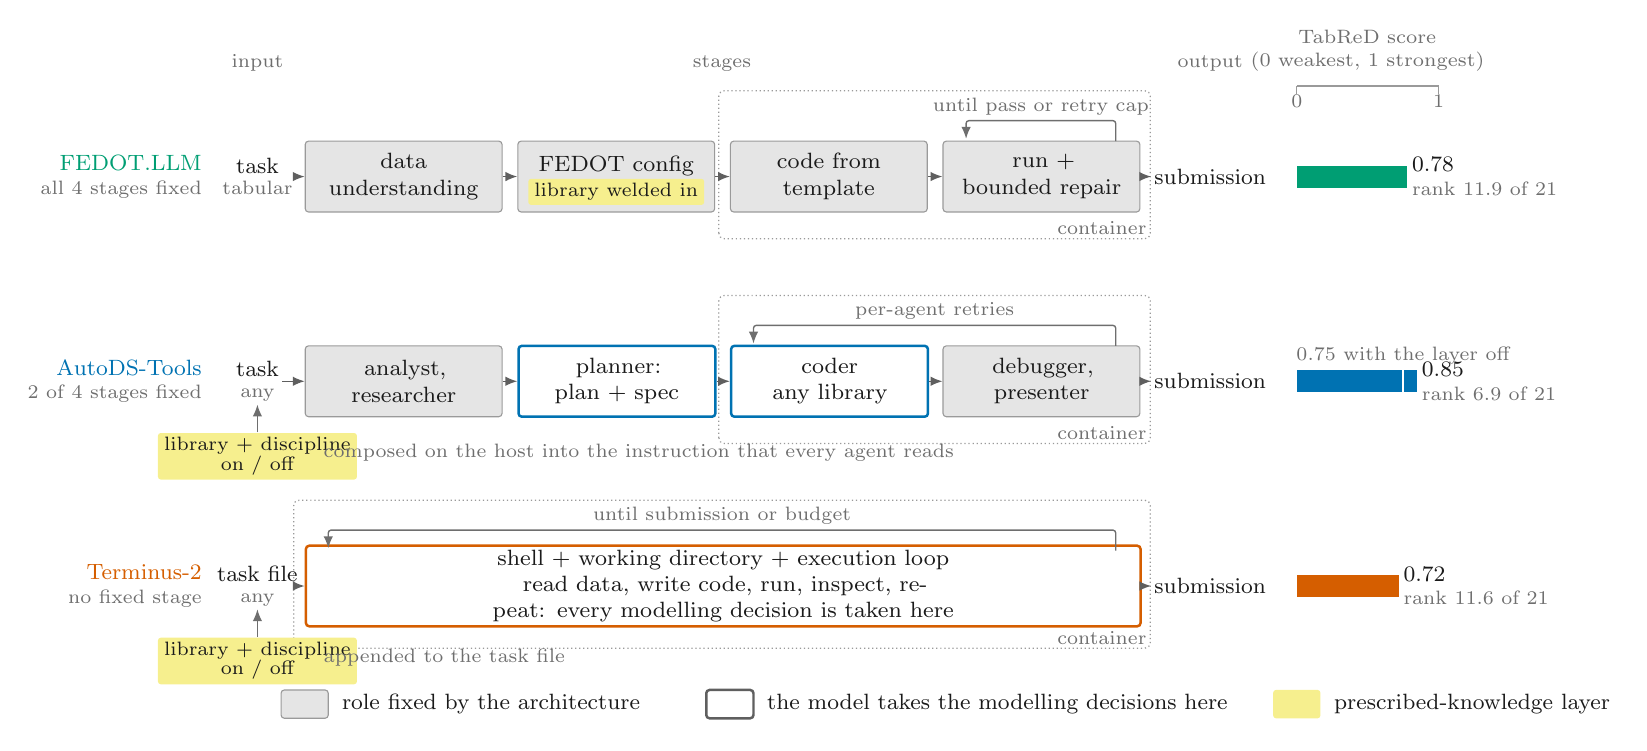
\begin{tikzpicture}[x=1mm,y=1mm, font=\footnotesize, text=ink,
  stage/.style = {draw=ctx, fill=black!10, rounded corners=1.2pt, line width=0.4pt,
                  minimum height=9mm, minimum width=25mm, text width=23.5mm,
                  align=center, inner xsep=0.5pt, inner ysep=1.5pt},
  free/.style  = {stage, fill=white, line width=0.9pt},
  chip/.style  = {fill=cLayer!60, rounded corners=1pt, inner xsep=2.2pt, inner ysep=1.6pt,
                  font=\scriptsize, align=center},
  io/.style    = {inner sep=1pt, align=center},
  arr/.style   = {-{Latex[length=1.5mm,width=1.2mm]}, draw=ink!70, line width=0.5pt},
  loop/.style  = {arr, draw=muted, rounded corners=1pt},
  env/.style   = {rounded corners=2pt, draw=ctx, densely dotted, line width=0.45pt},
  lbl/.style   = {font=\scriptsize, text=muted, inner sep=1pt, align=center},
  lane/.style  = {anchor=east, align=right, inner sep=0pt},
]
% ---- geometry ----------------------------------------------------------
\def\xLane{21}     % right edge of lane labels
\def\xTask{28}     % centre of the input node
\def\xA{34}\def\xB{61}\def\xC{88}\def\xD{115}   % left edges of the 4 stage columns
\def\wS{25}        % stage width
\def\xOut{149}     % centre of the output node
\def\xBar{160}     % score bar origin
\def\wBar{18}      % score bar span for score = 1
\def\yA{0}\def\yB{-26}\def\yC{-52}
\def\hRow{9}

% ---- header ------------------------------------------------------------
\node[lbl, anchor=south] at (\xTask,13) {input};
\node[lbl, anchor=south] at ({(\xA+\xD+\wS)/2},13) {stages};
\node[lbl, anchor=south] at (\xOut,13) {output};
\node[lbl, anchor=south, text width=30mm] at ({\xBar+\wBar/2},13)
     {TabReD score\\(0 weakest, 1 strongest)};
\draw[ctx, line width=0.4pt] (\xBar,11.5) -- ++(\wBar,0);
\foreach \t/\l in {0/0, 1/1} \draw[ctx, line width=0.4pt] ({\xBar+\t*\wBar},11.5) -- ++(0,-1)
   node[lbl, below, inner sep=0.3pt] {\l};

% ---- helpers -----------------------------------------------------------
% loop above the span [#1,#2] in row #3, label #4
\newcommand{\iterloop}[4]{%
  \draw[loop] ({#2-3},{#3+\hRow/2}) -- ({#2-3},{#3+\hRow/2+2.6}) -- ({#1+3},{#3+\hRow/2+2.6}) -- ({#1+3},{#3+\hRow/2+0.3});
  \node[lbl, anchor=south] at ({(#1+#2)/2},{#3+\hRow/2+2.9}) {#4};}
% dotted container frame around the span [#1,#2] in row #3
\newcommand{\envframe}[3]{%
  \begin{scope}[on background layer]
    \draw[env] ({#1-1.4},{#3-\hRow/2-3.4}) rectangle ({#2+1.4},{#3+\hRow/2+6.4});
  \end{scope}
  \node[lbl, anchor=south east, inner sep=1.2pt] at ({#2+1.4},{#3-\hRow/2-3.4}) {container};}
% score bar in row #1, value #2, colour #3, rank #4
\newcommand{\scorebar}[4]{%
  \fill[#3] (\xBar,{#1-1.4}) rectangle ({\xBar+#2*\wBar},{#1+1.4});
  \node[anchor=west, inner sep=1.5pt, align=left] at ({\xBar+#2*\wBar},#1)
       {#2\\[-1pt]{\scriptsize\color{muted}rank #4 of \nMethods}};}

% ============================ row 1: FEDOT.LLM ==========================
\node[lane, text=cFedot] at (\xLane,\yA) {FEDOT.LLM\\[-1pt]{\scriptsize\color{muted}all 4 stages fixed}};
\node[io] (t1) at (\xTask,\yA) {task\\[-2pt]{\scriptsize\color{muted}tabular}};
\node[stage, anchor=west] (a1) at (\xA,\yA) {data\\understanding};
\node[stage, anchor=west] (b1) at (\xB,\yA) {FEDOT config\\\phantom{x}};
\node[chip, anchor=south] at ([yshift=0.9mm]b1.south) {\Ktool{} welded in};
\node[stage, anchor=west] (c1) at (\xC,\yA) {code from\\template};
\node[stage, anchor=west] (d1) at (\xD,\yA) {run $+$\\bounded repair};
\node[io] (e1) at (\xOut,\yA) {submission};
\foreach \i/\j in {t1/a1,a1/b1,b1/c1,c1/d1,d1/e1} \draw[arr] (\i) -- (\j);
\iterloop{\xD}{\xD+\wS}{\yA}{until pass or retry cap}
\envframe{\xC}{\xD+\wS}{\yA}
\scorebar{\yA}{\nFedot}{cFedot}{\rkFedot}

% ============================ row 2: AutoDS-Tools ========================
\node[lane, text=cAuto] at (\xLane,\yB) {AutoDS-Tools\\[-1pt]{\scriptsize\color{muted}2 of 4 stages fixed}};
\node[io] (t2) at (\xTask,\yB) {task\\[-2pt]{\scriptsize\color{muted}any}};
\node[stage, anchor=west] (a2) at (\xA,\yB) {analyst,\\researcher};
\node[free, draw=cAuto, anchor=west] (b2) at (\xB,\yB) {planner:\\plan $+$ spec};
\node[free, draw=cAuto, anchor=west] (c2) at (\xC,\yB) {coder\\any library};
\node[stage, anchor=west] (d2) at (\xD,\yB) {debugger,\\presenter};
\node[io] (e2) at (\xOut,\yB) {submission};
\foreach \i/\j in {t2/a2,a2/b2,b2/c2,c2/d2,d2/e2} \draw[arr] (\i) -- (\j);
\iterloop{\xC}{\xD+\wS}{\yB}{per-agent retries}
\envframe{\xC}{\xD+\wS}{\yB}
\node[chip, anchor=north] (k2) at (\xTask,{\yB-6.5}) {\Ktool{} $+$ \Kdisc\\[-1pt]on / off};
\draw[arr, draw=muted] (k2.north) -- (t2.south);
\node[lbl, anchor=west, align=left] at ({\xA+2},{\yB-9.1}) {composed on the host into the instruction that every agent reads};
\scorebar{\yB}{\nAutoDS}{cAuto}{\rkAutoDS}
\draw[white, line width=0.6pt] ({\xBar+\nAutoDSOff*\wBar},{\yB-1.4}) -- ++(0,2.8);
\node[lbl, anchor=south] at ({\xBar+\nAutoDSOff*\wBar},{\yB+1.8}) {\nAutoDSOff{} with the layer off};

% ============================ row 3: Terminus-2 ==========================
\node[lane, text=cTerm] at (\xLane,\yC) {Terminus-2\\[-1pt]{\scriptsize\color{muted}no fixed stage}};
\node[io] (t3) at (\xTask,\yC) {task file\\[-2pt]{\scriptsize\color{muted}any}};
\node[free, draw=cTerm, anchor=west, minimum width={(\xD+\wS-\xA)*1mm}, text width={(\xD+\wS-\xA-3)*1mm}] (a3) at (\xA,\yC)
     {shell $+$ working directory $+$ execution loop\\read data, write code, run, inspect, repeat: every modelling decision is taken here};
\node[io] (e3) at (\xOut,\yC) {submission};
\draw[arr] (t3) -- (a3); \draw[arr] (a3) -- (e3);
\iterloop{\xA}{\xD+\wS}{\yC}{until submission or budget}
\envframe{\xA}{\xD+\wS}{\yC}
\node[chip, anchor=north] (k3) at (\xTask,{\yC-6.5}) {\Ktool{} $+$ \Kdisc\\[-1pt]on / off};
\draw[arr, draw=muted] (k3.north) -- (t3.south);
\node[lbl, anchor=west, align=left] at ({\xA+2},{\yC-9.1}) {appended to the task file};
\scorebar{\yC}{\nTerminus}{cTerm}{\rkTerminus}

% ---- legend --------------------------------------------------------------
\begin{scope}[shift={(\xA,-67)}]
  \node[stage, minimum width=6mm, minimum height=3.6mm, text width=5mm] at (0,0) {};
  \node[anchor=west] at (3.5,0) {role fixed by the architecture};
  \node[free, draw=ink!70, minimum width=6mm, minimum height=3.6mm, text width=5mm] at (54,0) {};
  \node[anchor=west] at (57.5,0) {the model takes the modelling decisions here};
  \node[chip, minimum width=6mm, minimum height=3.6mm] at (126,0) {};
  \node[anchor=west] at (129.5,0) {prescribed-knowledge layer};
\end{scope}
\end{tikzpicture}}
\caption{The three systems on one schematic. Grey stages have their role fixed
by the architecture; outlined stages are where the model takes the modelling
decisions. The yellow chip marks where the prescribed-knowledge layer enters:
welded into the FEDOT configuration, composed into the instruction that every
AutoDS-Tools agent reads, appended to the Terminus-2 task file. The loop above
a row shows what repeats and what ends it; the dotted frame is the container.
The right column gives the mean normalised TabReD score of
Section~\ref{sec:ceiling}, where 0 is the weakest and 1 the strongest of the
eighteen tuned methods on each task, and the average rank among the
\nMethods{} methods of Table~\ref{tab:leaderboard}. Fixed structure falls from
top to bottom; the score peaks in the middle row.}
\label{fig:systems}
\end{figure*}


\subsection{The instruction file and its two parts}
\label{sec:file}

AutoDS-Tools ships with an expert instruction file that is composed on the
host and prepended to the task statement every agent reads. In current
terminology it is an agent skill~\citep{li2026skillsbench}: standing
procedural instructions, independent of the task. It has two parts, which
we measure separately.
\begin{description}
  \item[Library instruction.] Which library to use for the task family: a
        dedicated tabular AutoML library (LightAutoML~\citep{vakhrushev2021lightautoml})
        for tabular data, a vision, graph or transformer library for the other
        modalities. It states that the library is pre-installed and forbids a
        fallback to general-purpose estimators.
  \item[Discipline instruction.] How to train and how to check oneself:
        the validation protocol, handling of temporal shift, leakage checks,
        comparison against a trivial predictor, allocation of the time budget,
        the prohibition of degenerate submissions, and advice on training
        time.
\end{description}
On a tabular task the file is about 5$\times$ as long as the task statement,
and the library instruction is about a quarter of it. An ablation that
switches the whole file at once cannot tell the two parts apart.

In FEDOT.LLM the library instruction is the workflow itself: every task goes
through FEDOT. Terminus-2 ships no instruction of its own, so we test the
file in a second harness by appending it to the task statement
(Table~\ref{tab:designpoints}).

\section{Experimental design}
\label{sec:design}

% STAGE 3: rewritten 8 September 2026.  Table~\ref{tab:arms} is new: one row
% per experimental arm, so the reader has a map of every run in the paper.

\subsection{Factors and arms}

The design varies five factors. \textbf{Architecture}: FEDOT.LLM, AutoDS-Tools,
Terminus-2. \Ktool{} and \Kdisc{}: each on or off, crossed on AutoDS-Tools and Terminus-2.
Terminus-2 ships no prescription of its own, so the halves of the AutoDS-Tools
layer are appended to its task file. \textbf{Backbone}:
\texttt{gemma-4-31b-it} throughout. AutoDS-Tools and Terminus-2 are also run
on a smaller model of the same family, \texttt{gemma-4-26b-a4b-it}, and on a
larger one from another family, \texttt{glm-4.7}, because the Gemma family has
nothing larger than 31B, so the upper point differs in family as well as in
size. Starting point: greenfield, where the agent receives the task statement alone,
and improve-a-baseline, where it also receives a working training script. Provisioning, the container image, is varied once, on Terminus-2. Swapping the
stock image for the enriched one changes the installed libraries and leaves the
instruction unchanged. Table~\ref{tab:arms} lists every arm these factors produce, with
the number of trials and the section that reports it.

\begin{table*}[t]
\centering
\caption{Every experimental arm in the paper. A trial is one attempt at one task; TabReD arms cover eight tasks, MLAgentBench arms the ten tasks of the benchmark, of which eight could be run three times on our hardware (Section~\ref{sec:coverage}). Stock: the benchmark's own image; enriched: the image built for AutoDS-Tools, with the libraries its layer names. Welded in: the library choice is fixed by the architecture (Section~\ref{sec:axis}); trimmed: the discipline half without its two clauses about training time (Section~\ref{sec:kdiscterm}). FEDOT image: the image built for FEDOT.LLM (Section~\ref{sec:deviations}).}
\label{tab:arms}
\footnotesize
\setlength{\tabcolsep}{4pt}
\begin{tabular}{lllllrl}
\toprule
System & Benchmark & Layer & Image & Backbone & Trials & Reported in \\
\midrule
FEDOT.LLM    & TabReD & welded in & FEDOT image & gemma-4-31b & 24 & \S\ref{sec:halfrange} \\
Terminus-2   & TabReD & none & stock & gemma-4-31b & 24 & \S\ref{sec:halfrange} \\
Terminus-2   & TabReD & none & enriched & gemma-4-31b & 24 & \S\ref{sec:matched} \\
Terminus-2   & TabReD & none, \Kdisc{}, \Ktool{}, both, \Kdisc{} trimmed & enriched & gemma-4-31b & $5\times24$ & \S\ref{sec:kdiscterm} \\
Terminus-2   & TabReD & none & enriched & gemma-4-26b-a4b, glm-4.7 & $2\times24$ & \S\ref{sec:modelaxis} \\
AutoDS-Tools & TabReD & none, \Kdisc{}, \Ktool{}, both & enriched & gemma-4-31b & $4\times24$ & \S\ref{sec:halfrange}, \S\ref{sec:grid} \\
AutoDS-Tools & TabReD & both & enriched & gemma-4-26b-a4b, glm-4.7 & $24+8$ & \S\ref{sec:modelaxis} \\
\midrule
AutoDS-Tools & MLAgentBench & none & enriched & gemma-4-31b & 30 & \S\ref{sec:headtohead}, \S\ref{sec:signflip} \\
AutoDS-Tools & MLAgentBench & both & enriched & gemma-4-31b & 30 & \S\ref{sec:signflip} \\
Terminus-2   & MLAgentBench & none & stock & gemma-4-31b & 24 & \S\ref{sec:headtohead} \\
FEDOT.LLM    & MLAgentBench & welded in & stock & gemma-4-31b & 2 & \S\ref{sec:coverage} \\
\midrule
AutoDS-Tools & three case studies & maximal, hand-written & enriched & gemma-4-31b & 3 & \S\ref{sec:cases} \\
Terminus-2   & three case studies & none, maximal & enriched & gemma-4-31b & $2\times9$ & \S\ref{sec:cases} \\
FEDOT.LLM    & two tabular cases & welded in & FEDOT image & gemma-4-31b & $2\times3$ & \S\ref{sec:cases} \\
\bottomrule
\end{tabular}
\end{table*}

\subsection{Benchmarks and reference points}
\label{sec:benchmarks}

\textbf{TabReD} contributes eight real-world tabular tasks with temporal
splits~\citep{rubachev2024tabred} and a published reference table of eighteen
methods: gradient boosting implementations~\citep{chen2016xgboost,ke2017lightgbm,prokhorenkova2018catboost},
tabular deep learning architectures, ensembles and retrieval-augmented models,
each tuned with Optuna~\citep{akiba2019optuna} on the official validation split
and averaged over fifteen seeds. Metrics are ROC-AUC for classification and
RMSE in raw target units for regression. The benchmark ships no agentic
protocol, so tasks are solved from scratch: this is the greenfield condition.
Every TabReD result in the paper is read against the reference table in two
ways: as an average rank among the published methods and the agents, and on a
normalised scale. For a task $j$ with score $s$ the normalised score is
$n_j(s) = (s - w_j)/(b_j - w_j)$, where $w_j$ and $b_j$ are the weakest and the
strongest published values on that task, so that $0$ is the weakest and $1$ the
strongest published method; for RMSE the weakest value is the largest. The mean
over the eight tasks has no floor, so a system below the weakest published
method on one task can score below $0$ there.

\textbf{MLAgentBench} contributes ten tasks spanning tabular, text, vision and
graph data~\citep{huang2024mlagentbench}. Each supplies a working but weak
training script and asks the agent to improve it: this is the
improve-a-baseline condition. MLAgentBench publishes no reference table, and the literature offers none at
the granularity we would need. MLAgentBench scores therefore stay in each
task's own metric, with no external ceiling to normalise against. Every MLAgentBench number in the paper compares two of our own runs under
identical conditions, for example AutoDS-Tools with the layer on against the
same system with it off, or AutoDS-Tools against Terminus-2 on the same task.
The normalised scale of Section~\ref{sec:ceiling} is used for TabReD only.

\textbf{Three scientific case studies}, published studies with author-reported
baselines, test external validity outside benchmark conditions
(Section~\ref{sec:cases}). Their instructions prescribe more than any other condition in the paper: the
library, the featurisation, the leakage handling and the baseline to beat. They
are therefore the most heavily prescribed point on the axis of
Section~\ref{sec:axis}. Terminus-2 runs on the full instruction and on the same instruction with the
library section removed. The case studies thus cross tool prescription with
architecture a second time, after TabReD (Sections~\ref{sec:grid}
and~\ref{sec:kdiscterm}).

\subsection{Execution environment and provisioning}

All runs execute inside the Harbor framework~\citep{harbor2026}, which records
for every trial the submission, the scorer output, the number of attempts and
errors, the wall-clock time, the token counts and the monetary cost. Cost and
attempts are therefore reported alongside accuracy throughout.
All backbones were called through OpenRouter, under the identifiers
\texttt{google/gemma-4-31b-it}, \texttt{google/gemma-4-26b-a4b-it} and
\texttt{z-ai/glm-4.7}, at the providers' default sampling settings; the paper
sets no temperature or context limit of its own. Costs are the per-request
figures OpenRouter reports, checked against the key balance to within $1.5\%$
on one cell; for \texttt{gemma-4-31b-it} the list price was \$0.09 per
million input and \$0.34 per million output tokens. The hub jobs ran in July and August 2026 and
the repeats on our hardware in August and September 2026, under Harbor~0.22.

Because a tool prescription presupposes the tool (Section~\ref{sec:axis}), we
state the container contents per arm. In the leaderboard arm Terminus-2 runs
on the benchmark's stock image, which ships the standard numerical and
data-frame libraries on Python~3.13. AutoDS-Tools requires the libraries its
prescription names and runs on an enriched image with them on Python~3.12.
FEDOT.LLM runs on an image built for it, with FEDOT and its dependencies on
Python~3.10. Data, splits, metrics and backbone are identical across arms; the
installed library set is not, and Section~\ref{sec:matched} measures what it is
worth.

The same applies to the instruction. Each system enters the leaderboard as it
is shipped: Terminus-2 with the task statement alone, FEDOT.LLM through a
pipeline whose tool choice is welded in, AutoDS-Tools with its
prescribed-knowledge layer applied. A row of Table~\ref{tab:leaderboard}
therefore compares deployed systems, and two further arms isolate the
architecture: AutoDS-Tools with the layer switched off, run as a full
$2\times2$ over \Ktool{} and \Kdisc{}, and Terminus-2 on the enriched image.

\subsection{Noise floor}

We measure a significance threshold and use it below. All three systems were
run three times on every TabReD task, and they do not share a floor.
Terminus-2's relative standard deviation across attempts ranges from
$\noiseTerminusMin\%$ to $\noiseTerminusMax\%$; AutoDS-Tools reproduces
itself an order of magnitude more tightly, from $\noiseAutoDSMin\%$ to
$\noiseAutoDSMax\%$, and on \allIdentAutoDS{} of its eight tasks every attempt
agrees to every digit; FEDOT.LLM agrees to every digit on \allIdentFedot{}
tasks and varies by up to $\noiseFedotMax\%$ on the rest. Between systems we
therefore treat a relative difference above $1\%$ as real, a threshold set by
the noisiest system, Terminus-2. Between configurations of AutoDS-Tools we
treat a difference above $0.1\%$ as real, a threshold set by its noisiest task.

All floors are optimistic, and for the same reason. On \bitIdentTerminus{} of
the eight tasks for Terminus-2, \bitIdentAutoDS{} for AutoDS-Tools and
\bitIdentFedot{} for FEDOT.LLM two attempts are bit-identical: the agent reproduced the same script, and on these
tasks the submission is a deterministic library call, so any two attempts that
reach the same call return the same number. The floors measure library
determinism as much as agent stability, and repeats carry less independent
information than their count suggests.

MLAgentBench has a noise floor nothing like the tabular one. Every cell was
run three times: sixty trials for AutoDS-Tools with the layer on and off and
twenty-four for Terminus-2. Three attempts of one cell
can span $\mlabOgbnOffLo$ to $\mlabOgbnOffHi$ in accuracy (AutoDS-Tools without
the layer on \texttt{ogbn-arxiv}) or $0.0844$ to $0.3846$ in micro-F1
(Terminus-2 on \texttt{fathomnet}). A difference on this benchmark is read as
real only when it exceeds a spread of that size, so Section~\ref{sec:mlab}
rests on cells in which a configuration produces no submission at all.
On TabReD a trial that exhausts its budget has written nothing; on
MLAgentBench the verifier scores whatever exists when the agent is stopped,
and such trials often submitted usable work (\texttt{clrs} scored $0.4118$
and $\mlabClrsOffHi$ on two of them), so the paper counts exhausting the
budget and returning nothing as separate events.

\subsection{Coverage}
\label{sec:coverage}

Coverage across the three systems is uneven, and every absence follows from
the architecture of FEDOT.LLM. All three systems attempt all eight TabReD
tasks; AutoDS-Tools and Terminus-2 attempt all ten MLAgentBench tasks, and
FEDOT.LLM two of the ten, because its architecture accepts tabular inputs
only: the segmentation, multi-label vision, graph and sequence tasks are
outside what it can express and would remain so after substantial
engineering. Its domain is the tabular core, the eight TabReD tasks plus
\texttt{house-price} and \texttt{spaceship-titanic}, and head-to-head
comparisons of all three systems are made there. That FEDOT.LLM can attempt
the fewest tasks follows from one decision: the pipeline is built around
FEDOT, a tabular AutoML library.

Two MLAgentBench tasks, \texttt{cifar10} and \texttt{imdb}, could not be
repeated, and the reason was measured. Sixteen attempts of sixteen exhausted
the agent budget without a submission at two concurrency settings, so
contention is not the cause. After the planning reports appear in the first
minute, a single Python process holds about eight cores continuously: a
training run. These two tasks are the heaviest to train and receive half the
budget of most others, $3600$\,s against $7200$, and their image installs the
CUDA build of PyTorch for a task that declares no accelerator, so training
falls back to the CPU. The five-epoch starter script finishes there; nothing
that improves on it does. Both tasks are omitted from every table that reports
three attempts per cell. The limit is our hardware.

\subsection{Deviations from the intended setup, and their measured cost}
\label{sec:deviations}

Two deviations from the intended design are known, and both are measured. The
first concerns the data. Earlier AutoDS-Tools runs on TabReD used a different
preparation: a $40{,}000$-row training slice spanning the official train and
validation splits, a test slice covering $16.7\%$ to $61.4\%$ of the official
test window, and an extra row-order column the official protocol withholds.
Those runs are excluded from every accuracy table in this paper; the
repair-loop counts of Section~\ref{sec:friction} come from them and are marked
as such. Table~\ref{tab:arms} uses a re-run of the same system through the
adapter that serves the full official splits, and both sets are released.
FEDOT.LLM and Terminus-2 ran through that adapter from the start. The earlier
comparison also differed in what was installed, the AutoDS-Tools arm carrying
the libraries its prescription names while the others used the stock image;
Section~\ref{sec:matched} closes that axis for Terminus-2; FEDOT.LLM runs on
its own image by construction. Its row is three attempts per task in the
system's full configuration: the best-quality preset, tuning on and a
$1200$\,s backend budget under the shared 8 cores, 16\,GB and $3600$\,s
ceiling. It reads the column types from the task schema, as the two agents
read them from the task text; with FEDOT's own type detection three of the
eight tasks returned no result. Four attempts that reached the ceiling while
a third job shared the machine were repeated at the concurrency of the rest,
and the repeats are the ones counted; every attempt is on the hub. The case
studies of Section~\ref{sec:cases} used a $2400$\,s budget under the same
ceiling.

The second concerns the image. The enriched image installs LightGBM as a dependency, but the base image and
the LightGBM wheel both lack an OpenMP runtime. The import therefore succeeds,
and the failure appears inside the fit as a broken worker pool that looks like
a modelling error. Forty-five trials met it: twenty-two of twenty-four AutoDS-Tools trials and
twenty-three of twenty-four Terminus-2 trials on the enriched image. All
forty-five diagnosed and repaired it in a single step, so it went unnoticed
until we read the traces.
Repeating the whole arm on a corrected image agrees to within $0.13\%$ on seven
tasks and $0.34\%$ on the eighth, so the defect cost no measurable accuracy. It
could still have distorted a crossed design, since the fault sits inside the
prescribed library and can strike only the cells where that prescription is
on. Every cell reported in the paper ran on the corrected image.

\section{Main results}
\label{sec:results}

% Remaster, 3 October 2026.  Main results = the three harnesses on
% TabReD against the published methods, on MLAgentBench head to head, on the
% case studies, and their cost.  Each subsection ends with a one-sentence
% Finding.  Ablations are in Section~\ref{sec:ablations}.

\subsection{TabReD: the harnesses among the tuned methods}
\label{sec:leaderboard}

Figure~\ref{fig:leaderboard} places the three harnesses among
the eighteen published methods; Table~\ref{tab:leaderboard} gives the raw
values. AutoDS-Tools reaches a mean normalised score of $\nAutoDS$, on par
with tuned LightGBM and below tuned XGBoost ($\nXGB$) and the strongest
published method, an MLP-PLR ensemble ($\nBest$). It is ahead of Terminus-2
($\nTerminus$) on \stshipAutoDSvsTerminusWins{} of 8 tasks.

\begin{figure*}[t]
\centering
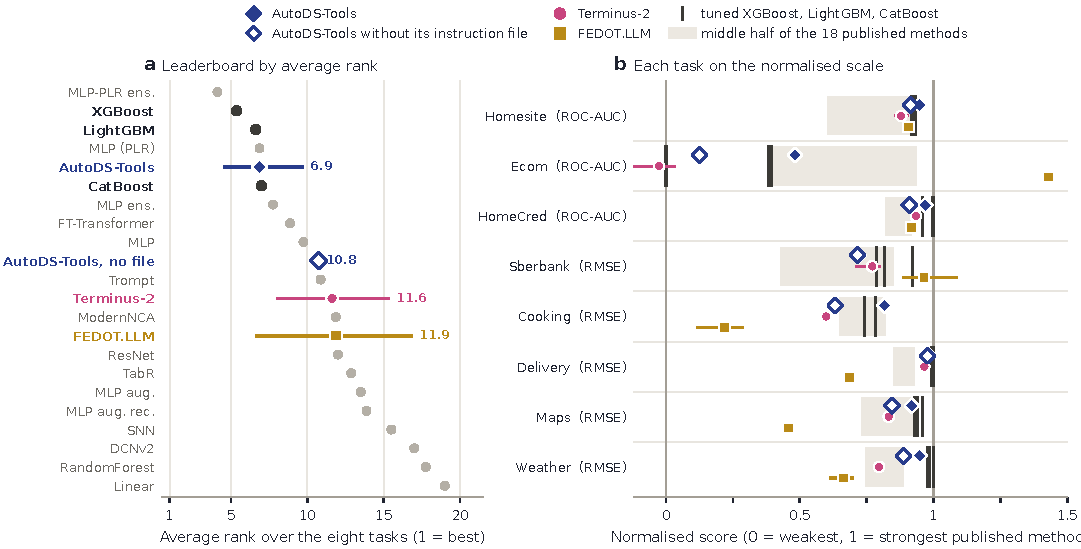
\includegraphics[width=\textwidth]{figures/fig_leaderboard.pdf}
\caption{The three harnesses among the eighteen tuned TabReD methods.
(a)~Average rank over the eight tasks; whiskers are 95\% bootstrap
intervals over tasks. (b)~Each task on the normalised scale; whiskers span
the three attempts. AutoDS-Tools is shown with its instruction file (filled) and
without it (open).}
\label{fig:leaderboard}
\end{figure*}
\begin{table*}[t]
\centering
\caption{Agent architectures placed in the TabReD leaderboard: full official temporal splits, the benchmark's metrics in raw units. Published rows are Optuna-tuned means over 15 seeds \citep{rubachev2024tabred}; agent rows use \texttt{gemma-4-31b-it}; agent rows are means over three attempts. Best per column in bold.}
\label{tab:leaderboard}
\small
\setlength{\tabcolsep}{3pt}
\begin{tabular}{lrrrrrrrrr}
\toprule
& \multicolumn{3}{c}{ROC-AUC $\uparrow$} & \multicolumn{5}{c}{RMSE $\downarrow$} & \\
\cmidrule(lr){2-4}\cmidrule(lr){5-9}
Method & Homesite & Ecom & HomeCred & Sberbank & Cooking & Delivery & Maps & Weather & Avg.\ rank \\
\midrule
\addlinespace[2pt]
\multicolumn{10}{l}{\itshape GBDT} \\
XGBoost & 0.9601 & 0.5763 & \textbf{0.8670} & 0.2419 & 0.4823 & 0.5468 & 0.1616 & 1.4671 & 5.4 \\
LightGBM & 0.9603 & 0.5758 & 0.8664 & 0.2468 & 0.4826 & 0.5468 & 0.1618 & \textbf{1.4625} & 6.6 \\
CatBoost & 0.9606 & 0.5596 & 0.8621 & 0.2482 & 0.4823 & \textbf{0.5465} & 0.1619 & 1.4688 & 7.0 \\
RandomForest & 0.9570 & 0.5764 & 0.8269 & 0.2640 & 0.4884 & 0.5959 & 0.1653 & 1.5838 & 17.8 \\
Linear & 0.9290 & 0.5665 & 0.8168 & 0.2509 & 0.4882 & 0.5579 & 0.1709 & 1.7679 & 19.0 \\
\addlinespace[2pt]
\multicolumn{10}{l}{\itshape Tabular DL} \\
MLP & 0.9500 & 0.6015 & 0.8545 & 0.2508 & 0.4820 & 0.5504 & 0.1622 & 1.5470 & 9.8 \\
SNN & 0.9492 & 0.5996 & 0.8551 & 0.2858 & 0.4838 & 0.5544 & 0.1651 & 1.5649 & 15.5 \\
DCNv2 & 0.9392 & 0.5955 & 0.8466 & 0.2770 & 0.4842 & 0.5532 & 0.1672 & 1.5782 & 17.0 \\
ResNet & 0.9469 & 0.5998 & 0.8493 & 0.2743 & 0.4825 & 0.5527 & 0.1625 & 1.5021 & 12.0 \\
FT-Transformer & 0.9622 & 0.5775 & 0.8571 & 0.2440 & 0.4820 & 0.5542 & 0.1625 & 1.5104 & 8.9 \\
MLP (PLR) & 0.9621 & 0.5957 & 0.8568 & 0.2438 & 0.4812 & 0.5527 & 0.1616 & 1.5177 & 6.9 \\
Trompt & 0.9588 & 0.5803 & 0.8355 & 0.2509 & 0.4809 & 0.5519 & 0.1624 & 1.5187 & 10.9 \\
\addlinespace[2pt]
\multicolumn{10}{l}{\itshape Ensembles} \\
MLP ens. & 0.9503 & 0.6019 & 0.8557 & 0.2447 & 0.4815 & 0.5494 & 0.1620 & 1.5186 & 7.8 \\
MLP-PLR ens. & \textbf{0.9629} & 0.5981 & 0.8585 & \textbf{0.2381} & \textbf{0.4806} & 0.5518 & \textbf{0.1612} & 1.4953 & 4.1 \\
\addlinespace[2pt]
\multicolumn{10}{l}{\itshape Training methodologies} \\
MLP aug. & 0.9523 & 0.6011 & 0.8449 & 0.2659 & 0.4832 & 0.5532 & 0.1631 & 1.5193 & 13.5 \\
MLP aug. rec. & 0.9531 & 0.5960 & 0.7453 & 0.2515 & 0.4834 & 0.5541 & 0.1636 & 1.5160 & 13.9 \\
\addlinespace[2pt]
\multicolumn{10}{l}{\itshape Retrieval-augmented} \\
TabR & 0.9487 & 0.5943 & 0.8501 & 0.2820 & 0.4828 & 0.5514 & 0.1639 & 1.4666 & 12.9 \\
ModernNCA & 0.9514 & 0.5765 & 0.8531 & 0.2593 & 0.4825 & 0.5498 & 0.1625 & 1.5062 & 11.9 \\
\midrule
\multicolumn{10}{l}{\itshape Agentic AutoML systems (this work)} \\
Terminus-2 \emph{(open harness)} & 0.9588 & 0.5585 & 0.8590 & 0.2491 & 0.4837 & 0.5482 & 0.1628 & 1.5247 & 11.6 \\
AutoDS-Tools \emph{(multi-agent)} & 0.9611 & 0.5800 & 0.8633 & 0.2515 & 0.4820 & 0.5474 & 0.1620 & 1.4783 & 6.9 \\
FEDOT.LLM \emph{(rigid pipeline)} & 0.9597 & \textbf{0.6200} & 0.8569 & 0.2398 & 0.4867 & 0.5620 & 0.1664 & 1.5651 & 11.9 \\
\bottomrule
\end{tabular}
\end{table*}


FEDOT.LLM ($\nFedot$) behaves differently from both agents. Its backend
search gives the best ROC-AUC of any method on \texttt{ecom-offers}
($\fedotEcomAuc$), and the same backend ranks 18th to 20th of 21 on four
regression tasks. Section~\ref{sec:ablations} shows how much of the
AutoDS-Tools lead comes from its instruction file.

\paragraph{Finding 1} With its instruction file, AutoDS-Tools is on par with tuned LightGBM
and ahead of Terminus-2 on \stshipAutoDSvsTerminusWins{} of 8 tasks
($p=\stshipAutoDSvsTerminusP$). FEDOT.LLM matches Terminus-2 on average and
differs from it on single tasks in both directions. None of the three reaches tuned XGBoost or the
strongest published method in this comparison.

\subsection{MLAgentBench: two harnesses from a working script}
\label{sec:mlab}

Table~\ref{tab:mlab} compares Terminus-2 with AutoDS-Tools on the eight
MLAgentBench tasks that repeat on our hardware, under one job, one verifier
and three attempts per task; AutoDS-Tools is shown with and without its
instruction file, and the comparison between harnesses uses the column
without it, since Terminus-2 carries none. AutoDS-Tools is the more accurate
of the two, taking \headWinsAutoDS{} of \headTasks{} tasks against
\headWinsTerminus{} for Terminus-2, with two ties: one task at the floor of
its metric and one inside the 5\% margin the table uses. Terminus-2 is the
faster and the less reliable: it uses about a third of the mean wall-clock
per trial, reaches its agent budget once in 24 trials where AutoDS-Tools
reaches it 13 times in 30 (the 30 include the two tasks that could not be
repeated), and ends without a submission in \headMissTerminus{} of 24
attempts against \headMissAutoDS{}. The spread
within a cell is large on this benchmark (Section~\ref{sec:stats}), so only
the win count and the submission counts are read as results.
\begin{table*}[t]
\centering
\caption{AutoDS-Tools with and without its prescribed-knowledge layer, and Terminus-2, on the eight MLAgentBench tasks that repeat on our hardware: one job, one verifier, three attempts per task. Mean, min and max are over the attempts that submitted; a superscript gives the number of submitting attempts where it is below three, and \emph{none} means no attempt submitted. Bold marks the better of AutoDS-Tools without the layer and Terminus-2 where the margin exceeds $5\%$. $\Delta$ is the change in mean score with the layer, divided by the larger of the two means, positive where the layer helps.}
\label{tab:mlab}
\footnotesize
\setlength{\tabcolsep}{3pt}
\begin{tabular}{llrrrrrrrrrr}
\toprule
 & & \multicolumn{3}{c}{AutoDS-Tools, layer off} & \multicolumn{3}{c}{AutoDS-Tools, layer on} & \multicolumn{3}{c}{Terminus-2} & \\
\cmidrule(lr){3-5}\cmidrule(lr){6-8}\cmidrule(lr){9-11}
Task & Metric & mean & min & max & mean & min & max & mean & min & max & $\Delta$ \\
\midrule
\texttt{clrs} & Ptr. acc. $\uparrow$ & \textbf{0.3909} & 0.3204 & 0.4404 & \multicolumn{3}{c}{none} & 0.1397$^{2}$ & 0.1330 & 0.1464 & \multicolumn{1}{c}{--} \\
\texttt{ogbn-arxiv} & Accuracy $\uparrow$ & \textbf{0.3866} & 0.2237 & 0.4790 & 0.5069 & 0.4334 & 0.5573 & 0.1606 & 0.0597 & 0.2655 & +0.24 \\
\texttt{spaceship-titanic} & Accuracy $\uparrow$ & \textbf{0.8074} & 0.8022 & 0.8131 & 0.8108 & 0.8080 & 0.8131 & 0.6590 & 0.5859 & 0.7059 & 0.00 \\
\texttt{house-price} & MAE $\downarrow$ & \textbf{15\,894.8} & 15\,529.7 & 16\,600.8 & 16\,433.4 & 16\,162.0 & 16\,904.2 & 21\,594.8$^{2}$ & 19\,422.1 & 23\,767.4 & -0.03 \\
\texttt{identify-contrails} & Dice $\uparrow$ & 0.0022 & 0.0000 & 0.0040 & 0.0478 & 0.0149 & 0.1137 & 0.0000$^{2}$ & 0.0000 & 0.0000 & +0.96 \\
\texttt{amp-parkinsons} & SMAPE $\downarrow$ & 62.2787$^{2}$ & 58.2113 & 66.3461 & 86.4637 & 81.7768 & 90.0803 & 60.4999$^{1}$ & -- & -- & -0.28 \\
\texttt{feedback} & MCRMSE $\downarrow$ & 0.8261 & 0.5403 & 1.2569 & \multicolumn{3}{c}{none} & \textbf{0.5279}$^{2}$ & 0.4972 & 0.5586 & \multicolumn{1}{c}{--} \\
\texttt{fathomnet} & micro-F1 $\uparrow$ & 0.1435$^{2}$ & 0.1428 & 0.1442 & \multicolumn{3}{c}{none} & \textbf{0.2440} & 0.0844 & 0.3846 & \multicolumn{1}{c}{--} \\
\bottomrule
\end{tabular}
\begin{tablenotes}\footnotesize
\item \texttt{identify-contrails} is counted as a tie between AutoDS-Tools and Terminus-2: both cells sit at the floor of the metric, and its $\Delta$ divides one small number by another and is not read as a result. Without the layer AutoDS-Tools takes 4 of the eight tasks against Terminus-2 and Terminus-2 2. Median trial: $6.1$ minutes for Terminus-2 against $10.9$ for AutoDS-Tools without the layer; means $19.1$ against $63.2$. Terminus-2 reached its agent budget once in $24$ trials, AutoDS-Tools $13$ times in $30$.
\end{tablenotes}
\end{table*}


\paragraph{Finding 2} From a working script, AutoDS-Tools takes
\headWinsAutoDS{} of \headTasks{} tasks and Terminus-2 \headWinsTerminus{};
Terminus-2 is three times faster on average and leaves three times as many attempts
without a submission.

\subsection{Three scientific case studies}
\label{sec:cases}

Three published studies with an author-reported baseline were turned into
Harbor tasks (Figure~\ref{fig:cases}, top row). Maize grain yield in the
Genomes-to-Fields trials~\citep{kick2023yield} is predicted for
location-years the model has never seen, with the authors' own split. Exit
state of jobs on the Fugaku supercomputer~\citep{antici2025fdata} is
predicted from what the scheduler knows at submission time; a constant
predictor scores $\caseFdataFloor$. Glass-transition temperature of polymers
in OpenPoly~\citep{wang2025openpoly} is predicted from a PSMILES string.
F-DATA and OpenPoly use random 80/20 splits, so their author figures come
from a different split: close in the case of F-DATA, distant in the case of
OpenPoly, where the authors used their full dataset.

\begin{figure*}[t]
\centering
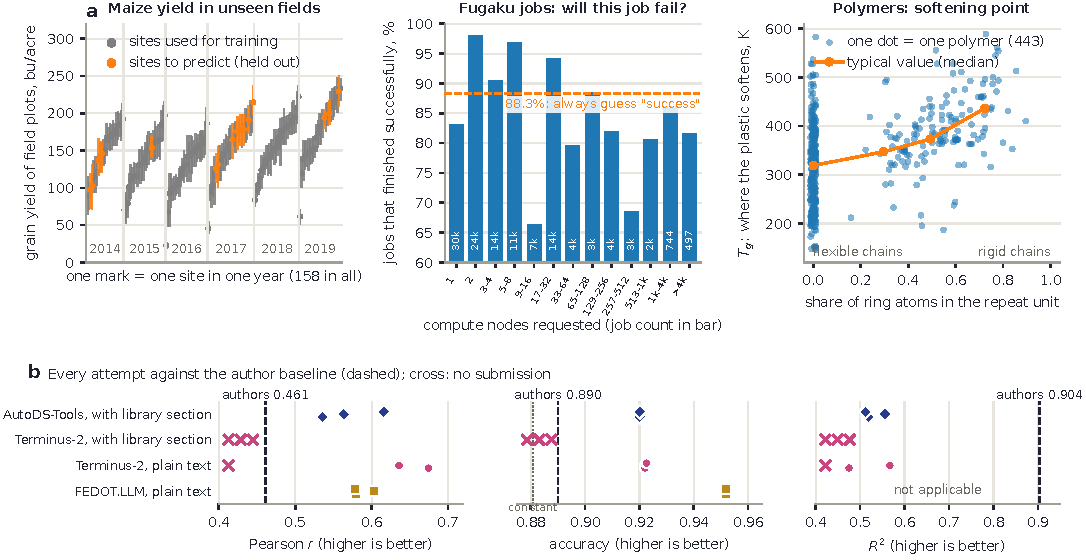
\includegraphics[width=0.96\textwidth]{figures/fig_cases.pdf}
\caption{The three case studies. Top: what each task asks, drawn from the
open data. Bottom: every attempt against the author baseline (dashed);
crosses mark attempts that ended without a submission.}
\label{fig:cases}
\end{figure*}

The task text was written for AutoDS-Tools and is the most prescriptive
condition in the paper: it names
LightAutoML~\citep{vakhrushev2021lightautoml} as the required library,
supplies a working snippet, lists the columns that leak the target,
describes the split and states the author baseline as the number to beat.
Every system has three attempts per case. AutoDS-Tools ran on that text
with its own instruction file off, since the text already names the library.
Terminus-2 ran on that text and on the same text with the library section
removed. FEDOT.LLM ran on the two tabular cases with a 40-minute backend
budget, its library being built in. Table~\ref{tab:cases} gives every row.
\begin{table*}[t]
\centering
\caption{Three scientific case studies, one row per system and task text: the published text with its library section, or the same text without it (plain). $n$ counts attempts that left a submission; mean, min and max are over those; minutes are the median agent time per attempt. Bold: the best system mean per case.}
\label{tab:cases}
\small
\setlength{\tabcolsep}{5pt}
\begin{tabular}{llllcrrrr}
\toprule
Case & Metric & System & Text & $n$ & mean & min & max & min/attempt \\
\midrule
Maize yield (G2F) & Pearson $r$ $\uparrow$ & \emph{authors} & & & 0.461 & & & \\
 & & AutoDS-Tools & with library section & 3/3 & 0.572 & 0.536 & 0.616 & 14.1 \\
 & & Terminus-2 & plain & 2/3 & \textbf{0.655} & 0.636 & 0.674 & 2.1 \\
 & & Terminus-2 & with library section & 0/3 & -- & -- & -- & 4.0 \\
 & & FEDOT.LLM & plain (library built in) & 3/3 & 0.587 & 0.578 & 0.603 & 52.8 \\
\midrule
Fugaku exit state (F-DATA) & Accuracy $\uparrow$ & \emph{authors} & & & 0.890 & & & \\
 & & AutoDS-Tools & with library section & 3/3 & 0.920 & 0.920 & 0.920 & 20.1 \\
 & & Terminus-2 & plain & 3/3 & 0.922 & 0.922 & 0.923 & 1.1 \\
 & & Terminus-2 & with library section & 0/3 & -- & -- & -- & 2.5 \\
 & & FEDOT.LLM & plain (library built in) & 3/3 & \textbf{0.952} & 0.952 & 0.952 & 45.4 \\
\midrule
Polymer $T_g$ (OpenPoly) & $R^2$ $\uparrow$ & \emph{authors} & & & 0.904 & & & \\
 & & AutoDS-Tools & with library section & 3/3 & \textbf{0.529} & 0.512 & 0.556 & 13.1 \\
 & & Terminus-2 & plain & 2/3 & 0.521 & 0.475 & 0.567 & 3.2 \\
 & & Terminus-2 & with library section & 0/3 & -- & -- & -- & 2.6 \\
\bottomrule
\end{tabular}
\begin{tablenotes}\footnotesize
\item AutoDS-Tools rows run the published text with the system's own instruction file off. FEDOT.LLM cannot act on the library section and has no molecular featurisation, so it has one row and was not run on OpenPoly. F-DATA: majority class scores 0.881. OpenPoly: the author figure is on the full dataset, ours on a subset with an 89-row test split, so that row is indicative only.
\end{tablenotes}
\end{table*}


Given the task text without the library section, Terminus-2 exceeded the
author baseline on maize (Pearson $r$ of $\caseTermPlainMaizeMin$ and
$\caseTermPlainMaizeMax$ against $\caseAuthorMaize$) and the author figure on
F-DATA ($\caseTermPlainFdataMean$ accuracy against $\caseAuthorFdata$), with
one to five minutes per attempt. On OpenPoly it chose RDKit~\citep{rdkit}
fingerprints and descriptors under XGBoost, the featurisation the authors
published.

With the library section in the text, Terminus-2 ended all
\caseTermPrescTotal{} attempts without a submission, against
\caseTermPlainLost{} of \caseTermPlainTotal{} without it. The mechanism is
that of Section~\ref{sec:abl-terminus}: the prescribed LightAutoML call takes
$\caseLamaFitFdataMin$ to $\caseLamaFitMaizeMin$ minutes on these tables, and
the agent declared the task complete after $1.5$ to $5.5$ minutes with the
fit still running. AutoDS-Tools completed all nine attempts on the same
text, its repair loop absorbing the wait. It is on par with Terminus-2 on
F-DATA and OpenPoly and below it on maize. FEDOT.LLM is the best system on
F-DATA, with balanced accuracy $\caseFedotPlainFdataBalancedAccuracy$
against $\caseTermPlainFdataBalancedAccuracy$ for Terminus-2 and
$\caseAutoDSFdataBalancedAccuracy$ for AutoDS-Tools.

\paragraph{Finding 3} Terminus-2 with the plain task text beat the author
baseline on maize, the one case with the authors' own split, and the author
figure on F-DATA, within minutes per attempt. The library instruction on
which AutoDS-Tools completed all nine attempts cost Terminus-2 all
\caseTermPrescTotal{} of its own.

\subsection{Cost and wall-clock}
\label{sec:cost}

\begin{table}[!t]
\centering
\caption{Cost and wall-clock per trial from the Harbor telemetry: means over trials of the trials' own cost, tokens and time. MLAB abbreviates MLAgentBench. Bold: the lowest value in its column within a benchmark.}
\label{tab:cost}
\scriptsize
\setlength{\tabcolsep}{2.5pt}
\begin{tabular}{llrrrrr}
\toprule
System & Bench & $n$ & \$/tr. & In/tr. & Out/tr. & Min/tr. \\
\midrule
Terminus-2 & TabReD & 24 & 0.0069 & 49\,969 & 2\,111 & \textbf{5.1} \\
AutoDS & TabReD & 24 & 0.0074 & 61\,606 & 5\,349 & 44.4 \\
FEDOT.LLM & TabReD & 24 & \textbf{0.0003} & \textbf{2\,680} & \textbf{155} & 33.1 \\
AutoDS ($K$ off) & MLAB & 30 & \textbf{0.0089} & \textbf{76\,463} & \textbf{5\,864} & 63.2 \\
AutoDS (shipped $K$) & MLAB & 30 & 0.0103 & 90\,439 & 6\,407 & 70.5 \\
Terminus-2 & MLAB & 24 & 0.4317 & 1\,989\,443 & 11\,873 & \textbf{19.1} \\
\bottomrule
\end{tabular}
\begin{tablenotes}\footnotesize
\item Distributions are right-tailed: the untreated AutoDS-Tools branch on MLAgentBench has a median of $10.9$ minutes against a mean of $63.2$, and one Terminus-2 trial (\texttt{feedback}, $571$ steps, \$8.71) is $84\%$ of its job, whose median trial cost \$0.033. FEDOT.LLM calls the model from inside its container, so its cost is its token count at list price.
\end{tablenotes}
\end{table}

A TabReD trial costs under a cent for any harness (Table~\ref{tab:cost}),
so the binding budget is wall-clock. On the same data adapter AutoDS-Tools
spends $\costRatioMin\times$ the mean wall-clock of Terminus-2
($\minAutoDSTabred$ against $\minTerminusTabred$ minutes per trial) for
$\costRatioDollars\times$ the money; its median trial is
$\rerunMedianMin$ minutes under the one-hour ceiling, and \rerunCut{} of
its 24 trials were cut by the ceiling, of which \rerunLost{} had no
submission to score. FEDOT.LLM spends
$\minFedotTabredMin$ to $\minFedotTabredMax$ minutes a task, almost all of
it backend search, with a few thousand model tokens per trial.

\paragraph{Finding 4} The API cost is negligible for all three harnesses
and wall-clock is the binding budget: AutoDS-Tools spends
$\costRatioMin\times$ the time of Terminus-2 and runs into the one-hour
ceiling in \rerunCut{} of 24 trials.

\section{Ablation studies}
\label{sec:ablations}

% Remaster, 3 October 2026.  Every factor the paper varies, one subsection
% each, summarised in Figure~\ref{fig:ablations}.  Each subsection ends with
% a one-sentence Finding.

Section~\ref{sec:results} compared the harnesses as shipped. This section
removes one factor at a time and measures what it was worth.
Figure~\ref{fig:ablations} summarises every ablation on two axes: the
paired difference in mean normalised score over the eight TabReD tasks, and
the share of trials that ended without a submission. Table~\ref{tab:grid}
and Table~\ref{tab:kdiscterm} give the per-task and per-cell numbers.

\begin{figure*}[t]
\centering
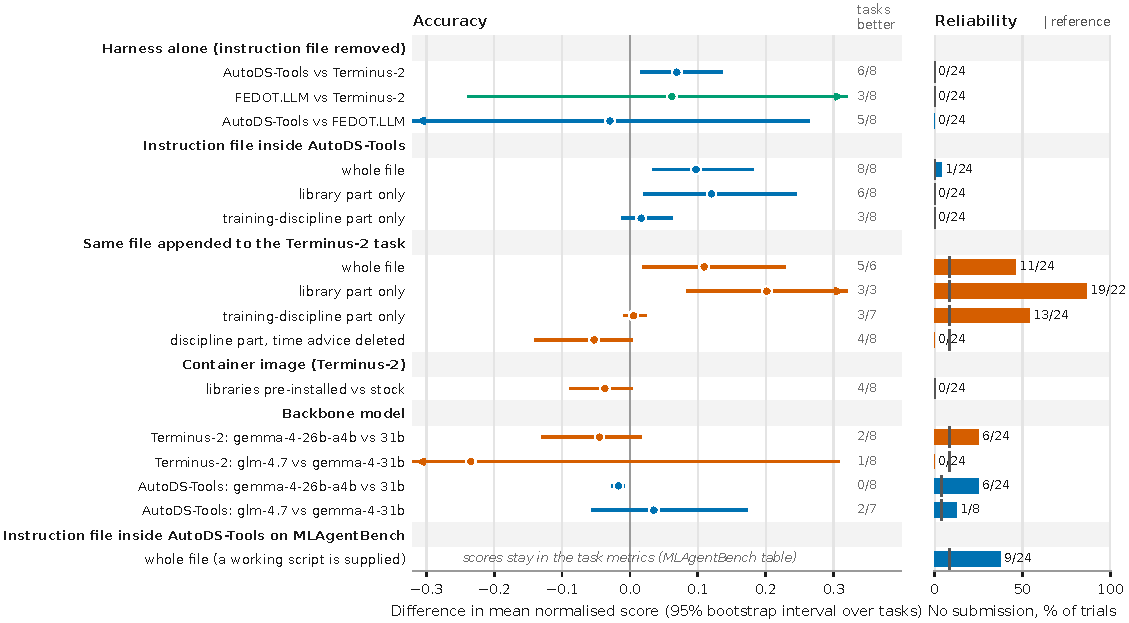
\includegraphics[width=\textwidth]{figures/fig_ablations.pdf}
\caption{Every factor the paper varies. Left: paired difference in mean
normalised score on TabReD (first configuration minus second), with the
95\% bootstrap interval over tasks and the number of tasks on which the
first is better. Right: trials that ended without a submission, with the
reference configuration as a tick. Arrows mark intervals that leave the
axis.}
\label{fig:ablations}
\end{figure*}

\subsection{Harness alone: the instruction file removed}
\label{sec:abl-harness}

With the instruction file switched off, AutoDS-Tools scores $\nAutoDSOff$
on the normalised scale, between Terminus-2 ($\nTerminus$) and FEDOT.LLM
($\nFedot$). On the same image, AutoDS-Tools without the file is ahead of
Terminus-2 on \starchAutoDSvsTerminusWins{} of 8 tasks by
$\starchAutoDSvsTerminusDiff$ (interval $\starchAutoDSvsTerminusLo$ to
$\starchAutoDSvsTerminusHi$, $p=\starchAutoDSvsTerminusP$): a small and
consistent lead that does not reach significance. FEDOT.LLM is level with
Terminus-2 on average ($p=\stshipFedotvsTerminusP$) and differs from it on
single tasks in both directions, from $+1.46$ on \texttt{ecom-offers} to
$-0.38$ on \texttt{cooking-time}.

\paragraph{Finding 5} Without the instruction file, the mean scores of the
three harnesses are close and no pairwise difference reaches $p<0.05$. The
harnesses still behave differently task by task: AutoDS-Tools is slightly
and consistently ahead of Terminus-2, and FEDOT.LLM varies most.

\subsection{The instruction file inside AutoDS-Tools}
\label{sec:abl-file}

Table~\ref{tab:grid} crosses the two parts of the file on AutoDS-Tools: four
cells of 24 trials on one image, one machine and one concurrency setting,
differing in the instruction file and in nothing else. The whole file lifts
the normalised score from $\nAutoDSOff$ to $\nAutoDS$, improving all eight
tasks ($\stfileBothDiff$, interval $\stfileBothLo$ to $\stfileBothHi$,
$p=\stfileBothP$). The library instruction alone lifts it to $\nGridTool$
(\stfileToolWins{} of 8 tasks, $p=\stfileToolP$), on par with tuned
XGBoost ($\sttoolVsXGBDiff$, $p=\sttoolVsXGBP$) and the best cell in the
paper; adding the discipline instruction on top changes it by
$\stbothVsToolDiff$ ($p=\stbothVsToolP$). The discipline instruction alone
lifts it to $\nGridDisc$ (\stfileDiscWins{} of 8, $p=\stfileDiscP$).
The traces show what the library instruction changes: with it,
AutoDS-Tools calls LightAutoML~\citep{vakhrushev2021lightautoml} in all 24
trials of both cells, and without it writes LightGBM, XGBoost or CatBoost by
hand in all 24 trials of both cells (Section~\ref{sec:spontaneous}). In the task metrics the library instruction improves the
mean by $\gridToolMeanU\%$, the discipline instruction by
$\gridDiscMeanU\%$ and both together by $\gridBothMeanU\%$, below the
$\gridSumHalvesU\%$ sum of the two. Two tasks carry most of the library
effect, \texttt{ecom-offers} ($\gridToolEcom\%$) and
\texttt{homecredit-default} ($\gridToolHomecredit\%$); no other task moves
by more than $\gridToolRestMax\%$. Of the $\gapAgentsShip$ by which
AutoDS-Tools as shipped leads Terminus-2, $\layerWorthNorm$ is therefore the
file and $\gapAgentsOff$ the harness.
\begin{table*}[t]
\centering
\caption{The prescribed-knowledge layer split into its halves on AutoDS-Tools over TabReD, twenty-four trials per cell on one image and one machine. The untreated cell is given in the task's own units; the other three as relative change against it, positive is better.}
\label{tab:grid}
\small
\setlength{\tabcolsep}{5pt}
\begin{tabular}{llrrrr}
\toprule
 & & untreated & \multicolumn{3}{c}{change against untreated, \%} \\
\cmidrule(l){4-6}
Task & Metric & cell & $K_{\text{tool}}$ only & $K_{\text{disc}}$ only & both \\
\midrule
\texttt{homesite-insurance} & ROC-AUC & 0.9600 & +0.10 & -0.03 & +0.12 \\
\texttt{ecom-offers} & ROC-AUC & 0.5649 & +3.68 & +1.24 & +2.67 \\
\texttt{homecredit-default} & ROC-AUC & 0.8559 & +0.79 & +0.20 & +0.86 \\
\texttt{sberbank-housing} & RMSE & 0.2516 & -0.31 & 0.00 & +0.07 \\
\texttt{cooking-time} & RMSE & 0.4835 & +0.47 & -0.04 & +0.30 \\
\texttt{delivery-eta} & RMSE & 0.5476 & 0.00 & -0.05 & +0.04 \\
\texttt{maps-routing} & RMSE & 0.1627 & +0.64 & +0.09 & +0.45 \\
\texttt{weather} & RMSE & 1.4968 & +0.14 & -0.41 & +1.24 \\
\midrule
mean over tasks & & & +0.69 & +0.12 & +0.72 \\
tasks improved & & & 6 of 8 & 3 of 8 & 8 of 8 \\
\bottomrule
\end{tabular}
\end{table*}


The two parts also cost differently. Naming the library shortens the
agent's search and lengthens the fit: the median trial goes from
$\gridNeitherMin$ minutes without instructions to $\gridToolMin$ with the
library named, and the API cost per trial falls from $\gridNeitherCost$ to
$\gridToolCost$ dollars. The discipline instruction does the opposite,
adding $\gridDiscCostPct\%$ to the cost and cutting the median trial to
$\gridDiscMin$ minutes. No cell lost more than one trial of 24.

\paragraph{Finding 6} Inside AutoDS-Tools the instruction file improves all
eight TabReD tasks ($p=\stfileBothP$) and accounts for $\layerWorthNorm$ of
the $\gapAgentsShip$ lead over Terminus-2. The library instruction carries
the effect by handing the modelling to LightAutoML, and alone reaches the
level of tuned XGBoost; the two parts gain less together than the sum of
their separate gains.

\subsection{The same file inside Terminus-2}
\label{sec:abl-terminus}

The file is composed on the host and reaches only its own agent, so to test
it in a second harness we appended the byte-identical parts to the
Terminus-2 task statement and ran 24 trials per cell on one machine, image,
backbone and concurrency setting (Table~\ref{tab:kdiscterm}); the part that
should be present appears in every trajectory, the part that should be
absent in none. Accuracy does not move: in the discipline cell every value
lands inside the spread of the cell without instructions, and the mean
difference is $\sttermDiscDiff$ (interval $\sttermDiscLo$ to
$\sttermDiscHi$). What moves is whether a trial produces an answer. Trials
ending without a submission go from \ktNeitherLost{} of 24 without
instructions to \ktDiscLost{} with the discipline instruction
($p=\ktPDiscVsNeither$), \ktToolLost{} of \ktToolTrials{} with the library
instruction ($p=\ktPToolVsNeither$) and \ktBothLost{} of 24 with both. None
is a timeout. The agent launches a fit in the foreground, sees a terminal
that has stopped producing output because its own job holds it, concludes
that reporting is broken and marks the task complete.
\begin{table}[t]
\centering
\caption{The instruction file appended to the Terminus-2 task statement on the eight TabReD tasks, 24 trials per cell on one machine, image and language model. Lost: trials ending with no submission. Steps and minutes are medians per trial.}
\label{tab:kdiscterm}
\footnotesize
\setlength{\tabcolsep}{3pt}
\begin{tabular}{lrrrrrrr}
\toprule
Cell & Trials & Lost & Tasks & Steps & Min & \$/trial & rel.\ \% \\
\midrule
none & 24 & 2 & 8/8 & 6 & 2.5 & 0.0029 & ref. \\
discipline & 24 & 13 & 7/8 & 18 & 14.1 & 0.0303 & -0.05 \\
discipline trimmed & 24 & 0 & 8/8 & 7 & 3.0 & 0.0044 & -0.69 \\
library & 22 & 19 & 3/8 & 14 & 10.2 & 0.0107 & +1.21 \\
both & 24 & 11 & 6/8 & 20 & 18.4 & 0.1172 & +1.13 \\
\bottomrule
\end{tabular}
\par\smallskip
\begin{minipage}{0.97\linewidth}\scriptsize The library cell lost two trials to a network fault and reports twenty-two. No cell had a timeout. Tasks: how many of eight returned a metric at least once. rel.\ \%: mean relative change against the cell without the file over the tasks that cell returns; the last two rows average over a surviving minority. Fisher's exact test on lost trials, two-sided: discipline against none $p=0.0013$; trimmed against discipline $p=2.6\times10^{-5}$; trimmed against none $p=0.49$; library against none $p=9.6\times10^{-8}$; library against both $p=0.0055$; a Holm correction changes no conclusion. Trimmed: the discipline instruction with its two paragraphs about training time removed.\end{minipage}
\end{table}


Two of the seven sections of the discipline instruction cause this. One
offers a hundred epochs as a starting budget and tells the agent to raise
it; the other tells it to assume it has ``hours, not minutes'' and that a
training phase finishing ``within a couple of minutes'' signals
undertraining. The median trial without instructions is two and a half
minutes of gradient-boosted trees and is not undertrained; the text was
written for convolutional and encoder models. Deleting those two sections
and keeping the other five loses no trial of 24, against \ktDiscLost{} with
the full instruction ($p=\ktPTrimVsDisc$) and \ktNeitherLost{} with none
($p=\ktPTrimVsNeither$), and returns the median trial to three minutes. With
the library instruction the fit is long because the prescribed library is
slow, and there the discipline instruction protects: the library instruction
alone loses \ktToolLost{} of \ktToolTrials{} trials, both together
\ktBothLost{} of 24 ($p=\ktPToolVsBoth$), because the discipline text tells
the agent that a long-running job is normal. AutoDS-Tools met none of this:
the same four cells inside its own harness lost none, none, none and one
trial of 24 (Section~\ref{sec:abl-file}).

\paragraph{Finding 7} Appended to Terminus-2, the file leaves accuracy
unchanged and ends \ktDiscLost{} of 24 trials without a submission with its
discipline part, \ktToolLost{} of \ktToolTrials{} with its library part and
\ktBothLost{} of 24 with both. For the discipline part, deleting two
paragraphs about training time restores every trial. The effect of an
instruction file has to be measured in each harness separately.

\subsection{The same file from a working script}
\label{sec:abl-script}

The two AutoDS-Tools column groups of Table~\ref{tab:mlab} ablate the whole
file over MLAgentBench, where every task starts from a working script. The
costly side is unambiguous: on \texttt{clrs}, \texttt{fathomnet} and
\texttt{feedback} the cell without the file scores in every attempt
($\mlabClrsOff$ pointer accuracy, $\mlabFathomnetOff$ micro-F1,
$\mlabFeedbackOff$ MCRMSE), and the cell with the file submits nothing in
any attempt, every attempt exhausting the task's agent budget. The paying
side is thin: only \texttt{ogbn-arxiv} gains by a margin that clears the
spread of either cell ($\mlabOgbnOff$ to $\mlabOgbnOn$);
\texttt{spaceship-titanic} and \texttt{house-price} do not differ beyond
their spreads, and \texttt{amp-parkinsons} moves against the file. The file
replaces a decision that the supplied script had already made, and on
MLAgentBench that replacement leaves no submission on \mlabWiped{} of
\mlabRepeated{} tasks and improves one.

The two benchmarks differ in tasks, metrics and budgets as well as in
starting point, so this is one factor observed across two protocols and we
do not add the win counts. The claim that holds inside each protocol is
this: from scratch, the file improves every TabReD task and loses no trial;
from a working script, it loses every attempt on \mlabWiped{} of
\mlabRepeated{} tasks.

\paragraph{Finding 8} The file that improves every TabReD task leaves no
submission on \mlabWiped{} of \mlabRepeated{} MLAgentBench tasks and helps
on one; what differs is whether a working default was already in place. The
count is a lower bound on the cost of the file, since the repair loop of
AutoDS-Tools absorbs part of it (Section~\ref{sec:friction}).

\subsection{Container image}
\label{sec:abl-image}

Running Terminus-2 on the enriched image built for AutoDS-Tools, same
tasks and three attempts each, changes the mean normalised score by
$\stimageDiff$ (interval $\stimageLo$ to $\stimageHi$,
$p=\stimageP$); \matchedWithin{} of the eight tasks stay inside the
harness's own noise floor, and the one outside it,
\texttt{sberbank-housing}, is one attempt that trained a thousand boosting
rounds without early stopping. Across all 24 trials the agent named none of
the three libraries the image pre-installs and went to gradient boosting by
hand, as on the stock image, where it had installed LightGBM itself. A
pre-installed library therefore changes the result only when an instruction
names it.

\paragraph{Finding 9} Pre-installing libraries that no instruction names
changes the mean normalised score by $\stimageDiff$, inside the noise of the
harness, and the agent uses none of them.

\subsection{Backbone}
\label{sec:abl-backbone}

Swapping the backbone under each harness, with tasks, image and instructions
unchanged, changes accuracy by less than the instruction file and changes
reliability by more. Under AutoDS-Tools
the smaller \texttt{gemma-4-26b-a4b} changes the normalised score by
$\stautodsSmallDiff$, worse on all eight tasks and by under one per cent in
the task metrics, and \texttt{glm-4.7} changes it by $\stautodsBigDiff$ (interval
$\stautodsBigLo$ to $\stautodsBigHi$, seven tasks scored). Under Terminus-2
the smaller model gives $\sttermSmallDiff$ and \texttt{glm-4.7}
$\sttermBigDiff$, the latter through one task: on \texttt{sberbank-housing}
the stronger model left the gradient-boosting default for a random forest
and lost $46\%$ of RMSE. On \texttt{ecom-offers} the same departure
produced the best ROC-AUC of any agent in this paper, $0.627$. Across the
same rows the price of a sweep of 24 trials varies \axPriceSpread$\times$,
from \$0.07 to \$0.93 under Terminus-2. Reliability moves in
opposite directions for the two harnesses: under Terminus-2 trials without
a submission fall from \axTerminusSmallLost{} of 24 to
\axTerminusRefLost{} to \axTerminusBigLost{} as the backbone strengthens;
under AutoDS-Tools they are lowest at the model the system was built
against (\axAutoDSRefLost{} of 24) and rise on both sides
(\axAutoDSSmallLost{} of 24 and \axAutoDSBigLost{} of the
\axAutoDSBigTrials{} trials we could afford), because a stronger model makes
the six agents exchange more text inside the same hour and more trials reach
the ceiling. Two models one generation older, \texttt{gemma-3-12b-it} and
\texttt{gemma-3-27b-it}, returned no usable submission in smoke trials on
\texttt{cooking-time} (the smaller emitted tool calls with empty arguments,
the larger left its submission in the wrong directory). There is a
capability floor below which neither harness produces a usable submission.

\paragraph{Finding 10} A backbone swap that changes the API cost
\axPriceSpread$\times$ moves accuracy by $\stautodsSmallDiff$ to
$\stautodsBigDiff$ under AutoDS-Tools and, under Terminus-2, by up to
$\sttermBigDiff$ through a single task; it moves reliability in opposite
directions for the two harnesses.

\section{Why: what the execution traces show}
\label{sec:mechanism}

% STAGE 3: rewritten 8 September 2026.

The results of the two previous sections agree with the statement that
constraint pays only where it removes a decision the model gets wrong. The
execution traces, which Harbor records for every trial, say why. This section
reads them for three things. Which tool does the unprescribed system reach
for, and does it tune it? Which clauses of the discipline half reach the
agent's behaviour? How often does prescription send the agent into repair?

\subsection{The unprescribed system picks the prescribed tool and never tunes it}
\label{sec:spontaneous}

If prescription pays only where the model's default is wrong, then on a family
where the default is already right it should be worth close to nothing. The
terminal traces of Terminus-2 test this without an ablation. Its instruction
names no library, only the task, the file layout, the output format and an
invitation to train and validate any model of its choosing. It fitted a
gradient-boosting model on every task in every attempt: LightGBM in
twenty-three of the twenty-four trials of Section~\ref{sec:matched} and XGBoost
in the remaining one. On the stock image it installed LightGBM itself on six of
the eight tasks. That is the family the tool prescription would have
named. On tabular data the prescription therefore restates the default. Inside
AutoDS-Tools it improves the task metric by $\gridToolMeanU\%$ on average over
the eight TabReD tasks, and inside Terminus-2 it changes nothing measurable.

The same traces locate the ceiling. The configuration is hand-written and
near-identical across tasks and attempts: $1000$ estimators in all twenty-four
trials, a learning rate of $0.05$ in twenty-three, early stopping on a holdout
in twenty-three, $31$ leaves in the nineteen that set a leaf count. No search
appears in any trace: no Optuna, no grid, no randomised search, no
cross-validated sweep. The gap to the published gradient-boosting rows is
therefore a gap in search: the harness picks the right tool unaided, the
baselines are Optuna-tuned over fifteen seeds, and the agent writes one
plausible configuration and stops. The per-task extraction is released with
the paper.

\subsection{The discipline half reaches the agent and leaves the score unchanged}
\label{sec:discipline}

Table~\ref{tab:grid} puts the discipline half of the layer at $\gridDiscMean\%$
on the task metric, averaged over the eight TabReD tasks. It does not say the half does nothing. The traces of the same four cells show that the discipline half reaches the
agent. Three
clauses ask it to compare against a trivial predictor, to allocate the time
budget before starting, and to keep the variant that validates best. All three behaviours appear in every trial of the two cells with the discipline
half on, and in no trial of the two cells with it off. The clause counts per cell are
released with the data package.

Two further clauses fail as a manipulation check, and both show why reading
one arm alone misleads. AutoDS-Tools inspects its submission in twenty-two of
twenty-four untreated trials and Terminus-2 in none, a habit of the
architecture that a cross-system comparison would credit to the instruction.
Early stopping is universal without the library and invisible with it,
because the prescribed library performs it internally. A signature shows that
an instruction reached the trace and leaves open whether it was carried out.

So the discipline block moves three behaviours from never to always and the
score by $\gridDiscMean\%$: the agent follows the block, and on tabular data
its own defaults were already adequate. The clause Terminus-2 never leaves a
trace of, inspecting the submission before finishing, exists to catch the
failure recorded in Section~\ref{sec:threats}, one constant label for a
$25{,}000$-row test set. Supplying the clause does not by itself pay: on
TabReD AutoDS-Tools inspects its submission in every trial and scores no
better for it, because there was nothing to catch.

\subsection{Prescription makes execution fail more often}
\label{sec:friction}

AutoDS-Tools contains a repair loop, invoked when execution fails. It is part
of the architecture and active in both branches, but it does not fire equally
often. The count comes from the earlier pair of jobs (eighteen tasks, one
attempt per cell, the earlier data preparation), since the loop was not
instrumented in the repeats, so we report a direction only. Across those thirty-six runs the loop fired eighteen times
with the layer against twelve without, in nine of eighteen runs against eight,
and the imbalance concentrates on the tasks where the prescription names a
specialised library: four invocations against none on \texttt{clrs} and three
against none on \texttt{amp-parkinsons}, both libraries whose interface the
agent then fails on.

Prescription therefore makes execution fail more often, and its net effect is
positive only where the prescribed tool gains enough to cover those failures.
We measure it inside a system that can recover from the errors it causes; in
a harness without a repair loop the losses are larger
(Section~\ref{sec:kdiscterm}). The same mechanism explains the disagreement
noted in Section~\ref{sec:related}: if knowledge injection bundles an
override that helps with one that hurts, and the mix of task families differs
between studies, aggregate ablations report inconsistent effects.

The trial artefacts name the clause behind the largest loss. The discipline
block tells the agent not to stop after ``an arbitrary small budget (5 or 15
epochs is almost always badly undertrained)'' and offers ``$\sim 100$
epochs'' as a starting point. On \texttt{clrs} the untreated branch chose $5$
to $30$ epochs, the range the clause forbids, reached $\mlabClrsOff$ pointer
accuracy and used $92$ minutes of a $120$-minute budget on one attempt; the
treated branch submitted nothing in three. A branch that already spends most
of the budget at $5$ to $30$ epochs cannot also honour a clause that names a
hundred, because the clause is written without reference to the budget the
task grants. The treated traces cannot be read, since the agent is killed at
the ceiling before it writes one.

\section{Discussion}
\label{sec:discussion}

% Remaster, 3 October 2026.

\subsection{What the results say about harness design}

Compared as shipped, the six-agent AutoDS-Tools ranks first on TabReD and
the workflow FEDOT.LLM and the minimal harness Terminus-2 are level. The
ablations attribute that order to two things that are separable from the
harness: the instruction file of one system and the backend search of
another. With the file removed, the three designs, from the fixed-stage
workflow to the open shell, reach the same region of the normalised scale,
and the differences between them equal the range a single harness covers
over its own attempts. Three designs cannot fix the shape of a curve, so we
do not claim that a designed middle ground would beat all three. What the
data support is narrower: on tabular tasks with a mid-size open model, the
choice of harness changes accuracy by less than the choice of attempt, and
changes reliability, wall-clock and the set of tasks a system can attempt
at all.

The instruction file is what changes accuracy, and the ablations show its
limits. It pays inside the harness it was written for, from
scratch, on the task family whose library it names. Moved to another
harness it ends half or more of the trials; applied where a working script
already exists it ends whole tasks. Both failures trace to specific sentences, the
advice on training time and the instruction to replace the supplied tool,
and both are invisible to an ablation that switches the file as one block.
This is also the reading we propose for the disagreement among published
ablations of instruction files and retrieved knowledge: a file measured in
one harness, from one starting point, has not been measured in another.

What separates every configuration from the strongest published method is
search. The agents choose the right model family unaided and write one
configuration; the reference methods are Optuna-tuned over fifteen seeds.
The one harness that searches, FEDOT.LLM, beats every published method on
the task where model choice matters most and is level with Terminus-2 over
the eight. Search over models and hyperparameters is a known, cheap addition
to any of the three harnesses, and the traces say it is the first thing to
add.

\subsection{Guidance for practitioners}

The results give one rule per situation. When a strong tuned baseline
exists, use it: the best cell in the paper is level with tuned XGBoost and
every cell is below the strongest published method. For a tabular task from
scratch with accuracy first and an hour per task acceptable, use
AutoDS-Tools with its instruction file. For a first pass over a new
scientific dataset in minutes per attempt, use Terminus-2 with the task text
alone, which beat two author baselines and found the published
featurisation on OpenPoly. Where search over a fixed backend pays, use
FEDOT.LLM, best of the three on \texttt{ecom-offers} and on F-DATA. When a
working script is supplied, add no library instruction. Two rules hold
across at least two protocols: prescribe only the decision the model would
otherwise get wrong, and keep advice about training time out of the prompt
of any harness with a hard time limit.

\subsection{Limitations}
\label{sec:threats}

\emph{Repeats.} Published baselines are means over fifteen seeds; agent rows
are means of three attempts, and on \allIdentFedot{} of eight tasks the three
FEDOT.LLM attempts agree to every digit, so its spread is understated. With
eight tasks the paired tests have little power, and we state them alongside
the win counts and intervals for that reason.

\emph{Scorers that accept degenerate submissions.} The prohibition on
constant submissions belongs to the instruction file, so only the cell with
the file carried it, and any bias from the asymmetry works against that
cell. Both degenerate submissions we found belong to Terminus-2: on
\texttt{imdb} one label for all 25\,000 test rows, scored at exactly
$0.5000$ and excluded, and on \texttt{amp-parkinsons} one global value in
$61.5\%$ of rows, read as a partial fallback.

\emph{The repair loop.} AutoDS-Tools repairs failed executions more often
with the file than without (Section~\ref{sec:friction}), so it partially
masks the cost of the file. We report the counts without adjustment;
disabling the loop in both branches is the experiment we would run next.

\emph{The lost trial.} One of the 24 AutoDS-Tools trials on TabReD
reached the one-hour limit with nothing to score and is excluded, so
\texttt{homesite-insurance} rests on two attempts. Scoring that attempt at
the weakest published value would move the normalised mean of AutoDS-Tools
from $\nAutoDS$ to $\sensLostNorm$, still ahead of the other two
harnesses; the exclusion drops the slowest attempt of a system whose
failures fall on the tasks it finds hardest.

\emph{Data access.} Several MLAgentBench tasks use subsets of the original
data and none an official test split, so every comparison there is
internal. On TabReD the agents receive the labelled validation split
(Section~\ref{sec:benchmarks}), a small advantage that works against our
main conclusion.

\emph{The backbone.} The backbone ablation rests on three models, two from
one vendor, and one task family. A stronger model that reasons less
verbosely might not push the multi-agent system into the time limit at all,
and we cannot separate capability from verbosity with what we ran. The
finding that the instruction file outweighs a backbone swap is therefore
reported for this domain and these models.

\emph{Generality of the harnesses.} The three systems are one instance each
of a workflow, a multi-agent system and a minimal harness. A different
six-agent system or a different fixed-stage workflow could behave
differently; the claim is about these three, and about the method of
separating harness, instructions and backbone, which transfers.

\section{Conclusion}
\label{sec:conclusion}

% Remaster, 5 October 2026.  Shortened; numbers stay in the Findings.

We asked where the accuracy of LLM-agent AutoML comes from and measured
three candidate sources separately: the harness, the instruction file and
the backbone. One open-weight 31B model ran under three harnesses on eight
real-world tabular tasks with temporal splits, and eighteen
hyperparameter-tuned reference methods served as the yardstick.

With the instruction file removed, a fixed-stage workflow, a six-agent
system and a minimal shell agent lie within $\spanArch$ of each other on the
normalised scale, no more than the variation between attempts of one
harness, and no pairwise difference is significant. The harness does affect
reliability, wall-clock time and the set of tasks a system can attempt.

The instruction file accounts for the accuracy gain, and its effect depends
on the harness and on the starting point. Used from scratch inside the
harness it was written for, it improves all eight tasks and brings the
system on par with tuned LightGBM. Appended to another harness, it ends half
or more of the trials without a submission; where a working script already
exists, it leaves whole tasks without one. An instruction file is therefore
part of the system under test and must be evaluated in each harness and from
each starting point.

No agent searches over hyperparameters, and this separates every
configuration from the strongest published method. A leaderboard built
around one harness measures the instructions that ship with it as well as
the model. Two experiments follow from the traces and remain to be run:
adding hyperparameter search to each harness under the same budget, and
disabling the repair loop of AutoDS-Tools to measure the cost of the
instruction file without it.

\section*{Data availability}

\begin{sloppypar}
All tasks, the instruction file in every variant used, and every execution
trace behind these numbers are public. The benchmark adaptations and the instruction files are
on HuggingFace as \texttt{danil-e/harbor-datasets-tabred} and
\texttt{danil-e/harbor-datasets-mlab}; the tabular adapter is
\texttt{AaLexUser/harbor-tabred-adapter}. Trajectories, submissions, scorer
outputs and telemetry of the earlier jobs are on the Harbor hub under job
identifiers \texttt{7593cc7b}, \texttt{1a42d1fe}, \texttt{3113aba7} and
\texttt{56768b37}, and the FEDOT.LLM TabReD row under \texttt{77c2d2f8},
\texttt{374be194}, \texttt{b9de44ad} and \texttt{7768c071}, where the same
tasks and scorer appear under the dataset name \texttt{tabred-fedot-schema},
the copy built on the FEDOT image; the repeats are
released in the data package with the
consolidated metric table, the per-task tables behind every summary, the
learner extraction of Section~\ref{sec:spontaneous}, the telemetry of
Table~\ref{tab:cost}, the byte lengths and hashes of every instruction-file variant, and the scripts
that produce every table and figure.
\end{sloppypar}
\todo{repository DOI once deposited}

\section*{CRediT authorship contribution statement}

\textbf{Stanislav Chumakov:} Conceptualization, Methodology, Investigation,
Formal analysis, Software, Validation, Visualization, Writing -- original
draft, Writing -- review \& editing.
\textbf{Danil Ezhov:} Investigation (AutoDS-Tools experiments), Software,
Data curation.
\textbf{Aleksei Lapin:} Investigation (Terminus-2 experiments), Software.
\textbf{Pavel Marian:} Investigation (FEDOT.LLM experiments), Software,
Resources (experiment tracking in Harbor).
\textbf{Kirill Anpilov:} Investigation (scientific case studies), Data
curation (case-study selection and task construction).
\textbf{Nikolay O. Nikitin:} Conceptualization, Supervision, Project
administration, Funding acquisition, Writing -- review \& editing.

\section*{Declaration of competing interest}

The authors declare that they have no known competing financial interests or
personal relationships that could have appeared to influence the work reported
in this paper.

\section*{Declaration of generative AI and AI-assisted technologies in the manuscript preparation process}

During the preparation of this work the authors used Claude Code (Anthropic)
to assist with writing and debugging the scripts that run the experiments and
produce the tables and figures, and to edit and format the manuscript text.
All tables and figures are generated by those scripts from the deposited
results; no image was created or altered by a generative model. After using this tool, the authors
reviewed and edited the content as needed and take full responsibility for the
content of the published article.

\section*{Acknowledgements}
\todo{funding, compute, and people to thank}


\bibliographystyle{elsarticle-num}
\bibliography{refs}

\end{document}
